\documentclass[11pt]{article}

% ---------- packages ----------
\usepackage[utf8]{inputenc}
\usepackage[T1]{fontenc}
\usepackage{lmodern}
\usepackage[a4paper,margin=1in]{geometry}
\usepackage{amsmath,amssymb}
\usepackage{graphicx}
\usepackage{booktabs}
\usepackage{array}
\usepackage{caption}
\usepackage{subcaption}
\usepackage{float}
\usepackage{microtype}
\usepackage{enumitem}
\usepackage{titlesec}
\usepackage[table]{xcolor}
\usepackage[hidelinks]{hyperref}

\graphicspath{{figures/}}

% ---------- float tuning (many figures) ----------
\renewcommand{\topfraction}{0.92}
\renewcommand{\bottomfraction}{0.85}
\renewcommand{\textfraction}{0.07}
\renewcommand{\floatpagefraction}{0.78}
\setcounter{totalnumber}{6}
\setcounter{topnumber}{4}
\setcounter{bottomnumber}{4}

\captionsetup{font=small,labelfont=bf,width=0.95\textwidth}

% ---------- macros ----------
\newcommand{\degC}{\ensuremath{^{\circ}}C}
\newcommand{\Tcap}{T_{\mathrm{cap}}}
\newcommand{\Esum}{E_{\mathrm{hvac}}}
\newcommand{\sigpost}{\sigma_{\mathrm{post}}}
\newcommand{\R}{\mathbb{R}}
\newcommand{\code}[1]{\texttt{\small #1}}

\titleformat{\section}{\normalfont\large\bfseries}{\thesection}{0.6em}{}
\titleformat{\subsection}{\normalfont\normalsize\bfseries}{\thesubsection}{0.6em}{}

\setlength{\parskip}{2pt}

% =====================================================================
\begin{document}

\begin{titlepage}
\centering
\vspace*{0.6cm}
{\LARGE\bfseries A Physics-in-the-Loop Digital Twin with a Dual-Loop\\[4pt]
Control Framework for Safe, Energy-Optimal\\[4pt]
Data-Center Cooling\par}

\vspace{1.1cm}
{\large\bfseries Hoang-Huy Nguyen\textsuperscript{1,$\ast$}\par}
\vspace{0.5cm}
{\normalsize \textsuperscript{1}Digital Twin Dual-Loop Control Project\par}
{\normalsize \textsuperscript{$\ast$}Corresponding author: \href{mailto:huyfanne@gmail.com}{huyfanne@gmail.com}\par}

\vspace{1.0cm}
{\normalsize Manuscript draft --- June 2026\par}

\vspace{1.2cm}
\begin{minipage}{0.86\textwidth}
\small
\noindent\textbf{Abstract.}
Cooling typically accounts for 30--40\% of a data center's non-IT electricity, yet
the inlet-air temperature of every server is a hard safety constraint that operators
are unwilling to risk. We present a \emph{digital twin dual-loop control framework}
that recommends weekly cooling setpoints for a tropical, water-cooled hyperscale hall
while guaranteeing that no server inlet ever exceeds \(26\,\degC\). An \emph{inner
planning loop} treats a full-building EnergyPlus~9.5 model --- coupled in the loop
through Docker and BCVTB --- as the physical oracle: a coarse-to-fine beam search
proposes three global setpoints (supply-air temperature, CRAH airflow, and
chilled-water supply temperature), each candidate is scored by a complete
week-long physics simulation, and a three-layer safety gate rejects anything it cannot
\emph{prove} robust. An \emph{outer deployment loop} pre-validates the chosen plan,
expands it to 45 per-actuator commands, deploys it in shadow mode, measures the realized
week, and learns per-KPI bias and two uncertainties that feed back into both the search
margin and a worst-case robust ensemble; a slower physics-recalibration step corrects
the plant's fan-efficiency parameters from persistent energy residuals. Over six
consecutive deployed weeks the twin's weekly-energy prediction error fell from
\(1.33\%\) to \(0.10\%\), energy savings against the as-operated baseline ramped from
\(0\%\) to \(3.6\%\) --- released only as fast as measured confidence allowed --- and
\emph{zero} safety violations occurred (worst realized inlet \(25.60\,\degC\)).
We give the full physical and statistical formulation, including the energy and
recirculation models, the conditional-value-at-risk robustness gate, and the
empirical-Bayes uncertainty that sizes it, and we illustrate the operator-facing web
application that drives the loop.

\vspace{0.4cm}
\noindent\textbf{Keywords:} digital twin; data-center cooling; EnergyPlus co-simulation;
safe optimization; beam search; robust feasibility; conditional value-at-risk;
calibration; energy efficiency.
\end{minipage}

\vfill
\end{titlepage}

% =====================================================================
\section{Introduction}
\label{sec:intro}

Data centers consumed an estimated 1--2\% of global electricity in the mid-2020s, and
within a facility the cooling system is the dominant non-computing load, commonly
30--40\% of overhead power~\cite{barroso,greengrid,patterson}. The efficiency of a
center is summarized by its \emph{Power Usage Effectiveness} (PUE), the ratio of total
facility power to IT power; every reduction in cooling power moves PUE toward its ideal
value of~1. At the same time, cooling is a \emph{safety-critical} function: each server
draws air at an inlet whose temperature must stay within the envelope recommended by
ASHRAE Technical Committee~9.9~\cite{ashrae}. Exceeding the inlet limit risks thermal
throttling, accelerated hardware failure, and --- in the tail --- thermal shutdown of a
production hall. Operators therefore run cooling conservatively, leaving large but
\emph{unrealized} efficiency gains on the table because no recommendation can be trusted
that has not been shown to be safe.

This tension --- aggressive energy optimization versus an inviolable thermal constraint
under model and weather uncertainty --- is precisely what a \emph{digital
twin}~\cite{glaessgen} is suited to resolve. A high-fidelity physics model of the plant
can predict, before anything is actuated, what a proposed setpoint will do to both energy
and to the hottest server inlet in the hall. Prior data-center control work has explored
machine-learning surrogates~\cite{gao}, model-predictive control over learned
dynamics~\cite{lazic}, and reinforcement-learning testbeds built on EnergyPlus
itself~\cite{moriyama}. These approaches optimize well on average but treat the safety
constraint softly, or rely on a learned model whose extrapolation behaviour near the
constraint boundary is hard to certify. Our design takes the opposite stance: the
constraint is hard and is checked by the same first-principles building-physics engine,
EnergyPlus~9.5~\cite{energyplus,eplusref}, that the industry uses for design, coupled
\emph{in the loop} through the Building Controls Virtual Test Bed (BCVTB)~\cite{bcvtb}.

We make the following contributions.
\begin{enumerate}[leftmargin=1.4em,itemsep=2pt,topsep=2pt]
  \item \textbf{A dual-loop framework} that cleanly separates a fast \emph{inner planning
  loop} (forecast \(\rightarrow\) physics oracle \(\rightarrow\) search \(\rightarrow\)
  safety gate) from a slow \emph{outer deployment loop} (pre-validation \(\rightarrow\)
  expert approval \(\rightarrow\) shadow deploy \(\rightarrow\) measure \(\rightarrow\)
  learn), with EnergyPlus as the in-the-loop oracle on \emph{both} sides.
  \item \textbf{A complete physical and statistical formulation} of the controller: the
  hall-scoped energy objective, the recirculation mixing model that connects supply-air
  setpoints to server inlets, a coarse-to-fine beam search over three global setpoints
  broadcast to 45 actuators, and a three-layer safety architecture whose robustness is
  sized by an empirical-Bayes posterior uncertainty.
  \item \textbf{A measured, closed-loop demonstration} over six consecutive weekly
  cycles, in which prediction error, energy savings, and the safety record are reported
  from the live system rather than asserted, together with the operator-facing web
  application that makes the loop usable.
\end{enumerate}

The remainder of the paper is organized as follows.
Section~\ref{sec:overview} describes the physical plant and the dual-loop architecture.
Section~\ref{sec:formulation} gives the physical and mathematical formulation of the
oracle, the control parametrization, the objective, the forecaster, and the
recirculation model. Section~\ref{sec:search} details the beam-search optimizer and
the experiment establishing that the optimization is physically well-posed.
Section~\ref{sec:safety} presents the three-net robust safety gate.
Section~\ref{sec:outer} describes calibration and physics recalibration --- how the twin
learns. Section~\ref{sec:webapp} presents the web application and the operator workflow,
with screenshots. Section~\ref{sec:results} reports the six-week deployment results.
Section~\ref{sec:discussion} discusses limitations honestly, and
Section~\ref{sec:conclusion} concludes.

% =====================================================================
\section{System Overview}
\label{sec:overview}

\subsection{The physical plant}
The controlled facility is a seven-hall, water-cooled tropical data center modeled to
scale in EnergyPlus from its real zone geometry (Fig.~\ref{fig:building}). We control a
single production hall, designated \textbf{1F~2A}, which contains 22 computer-room air
handlers (CRAHs) serving \(\approx 2.0\,\mathrm{MW}\) of IT load and is served by a
\emph{shared} chilled-water plant (chillers, cooling towers, and pumps) common to the
building. The remaining halls are part of the simulation but are not actuated by the
planner.

\begin{figure}[t]
  \centering
  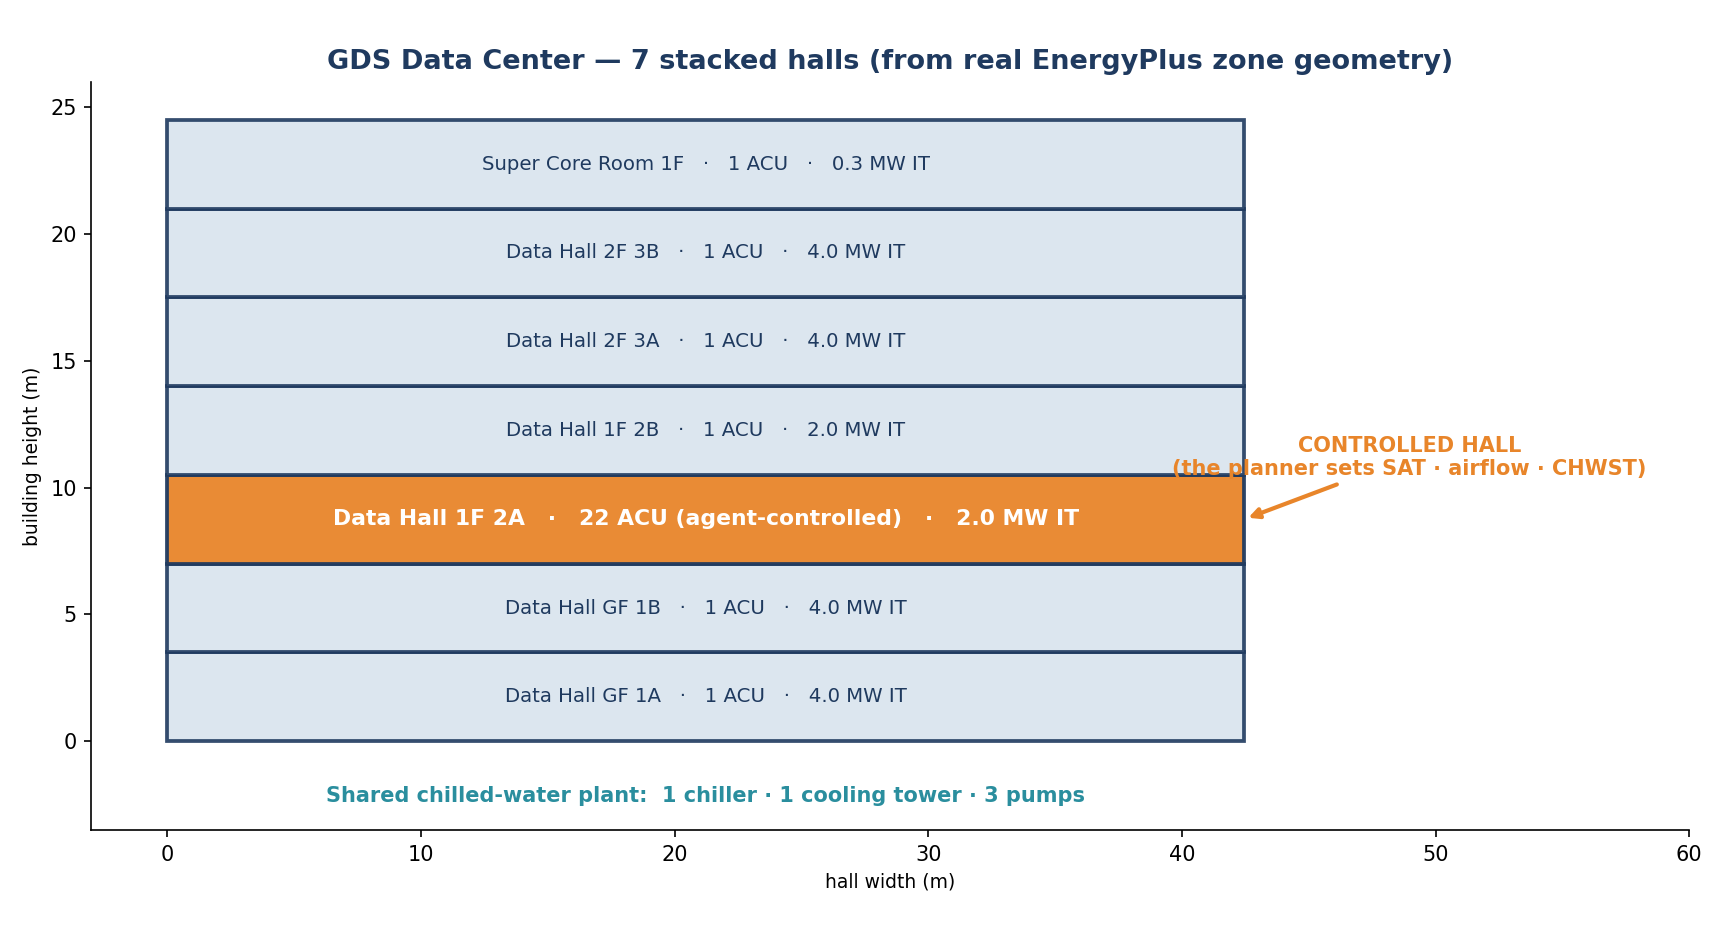
\includegraphics[width=\linewidth]{fig1_building.png}
  \caption{The modeled data center: seven stacked halls drawn to scale from the real
  EnergyPlus zone geometry. The orange hall (1F~2A) is the controlled hall --- 22
  agent-controlled CRAHs and \(\approx\!2.0\,\mathrm{MW}\) of IT load --- served by a
  shared chilled-water plant. The planner sets only this hall's supply-air temperature,
  airflow, and the chilled-water supply temperature.}
  \label{fig:building}
\end{figure}

Within the controlled hall (Fig.~\ref{fig:hall}), the racks are arranged in standard
hot-aisle/cold-aisle rows. The planner exposes only three \emph{global} setpoints, which
the building's control logic broadcasts to the individual actuators:
\begin{itemize}[leftmargin=1.4em,itemsep=1pt,topsep=2pt]
  \item \textbf{SAT} --- CRAH supply-air temperature, range \(20\)--\(26\,\degC\);
  \item \textbf{Airflow} --- CRAH supply airflow, range \(4.8\)--\(13.8\,\mathrm{kg/s}\) per ACU;
  \item \textbf{CHWST} --- chilled-water supply temperature, range \(13\)--\(19\,\degC\).
\end{itemize}
These three numbers expand to \(22\) SAT \(+\;22\) airflow \(+\;1\) CHWST \(=45\)
per-actuator commands (Section~\ref{sec:broadcast}). The overriding constraint is a
\textbf{hard cap of \(26\,\degC\) on every server inlet at every 15-minute step}.

\begin{figure}[t]
  \centering
  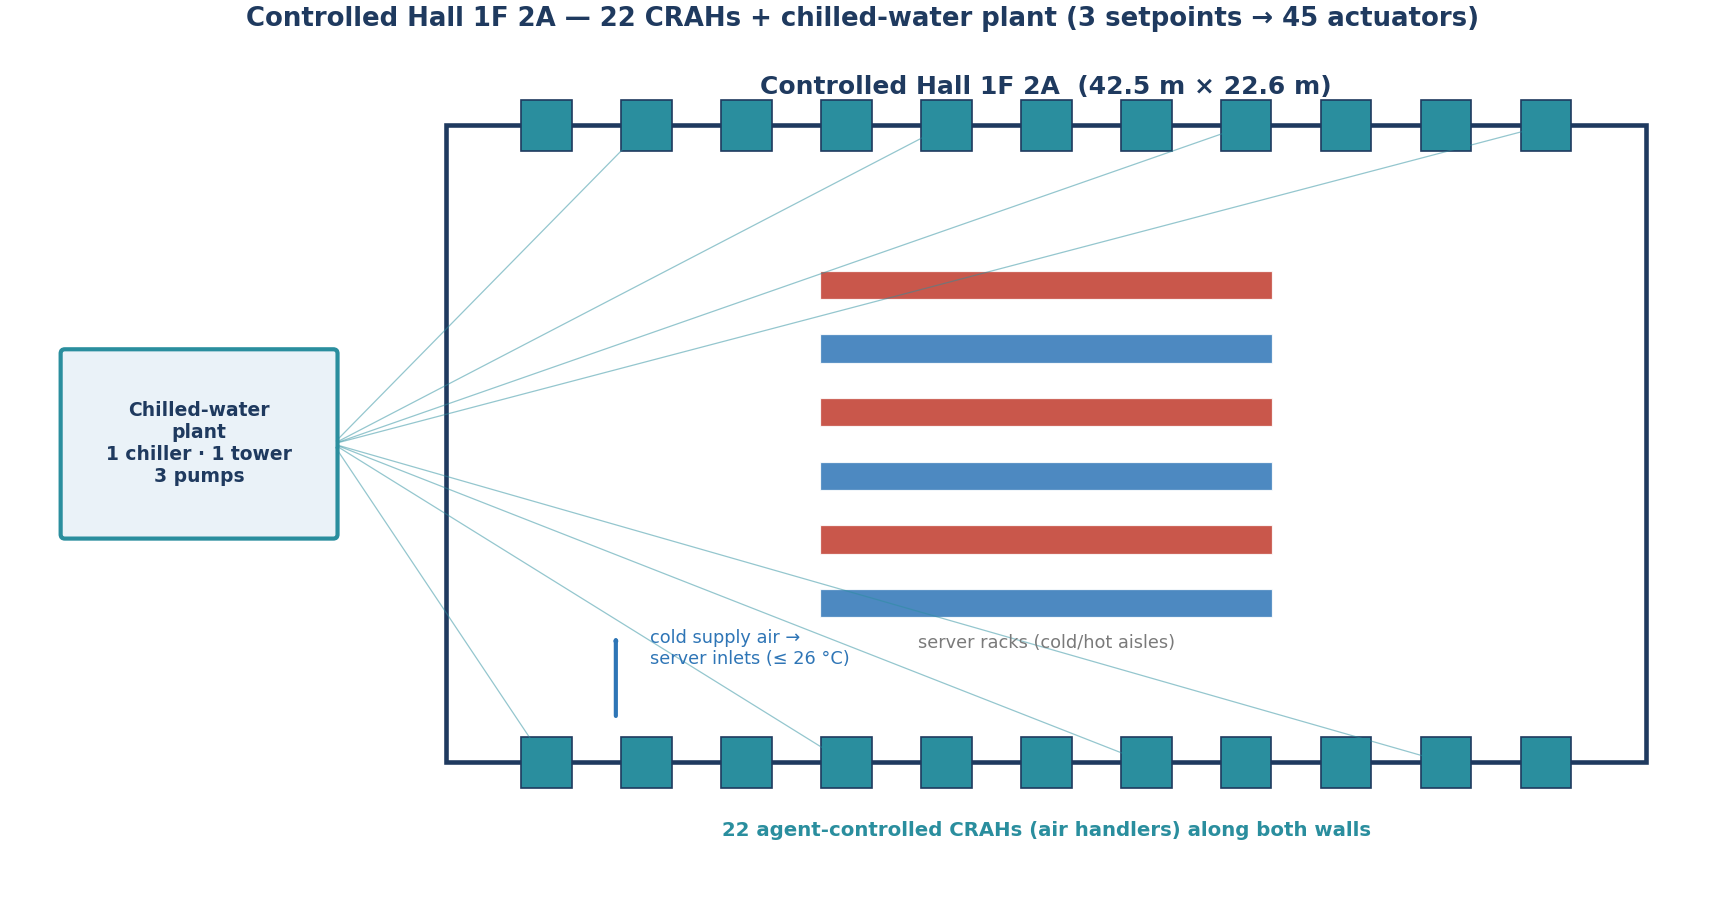
\includegraphics[width=\linewidth]{fig2_hall.png}
  \caption{Plan view of the controlled hall 1F~2A: hot-aisle/cold-aisle rack rows, 22
  CRAHs along the walls, and the shared chilled-water plant. The three global setpoints
  (SAT, airflow, CHWST) are broadcast to \(22+22+1=45\) actuators that deliver cold
  supply air to the server inlets, which must remain at or below \(26\,\degC\).}
  \label{fig:hall}
\end{figure}

\subsection{The dual-loop architecture}
The framework (Fig.~\ref{fig:arch}) is organized as two nested loops.

\emph{The inner planning loop} runs entirely in simulation. A \emph{forecaster} predicts
the coming week's IT load and weather; a \emph{beam search} proposes candidate setpoint
triples; an \emph{oracle} scores each candidate with a full-week EnergyPlus run; an
\emph{objective} converts each candidate's key performance indicators (KPIs) into a
scalar cost while a \emph{safety gate} rejects any candidate that violates --- or cannot
be proven to robustly satisfy --- the inlet cap. The result is a single recommended plan.

\emph{The outer deployment loop} closes the system to operations. The recommended plan is
\emph{pre-validated} by independent nominal and worst-case replays; an expert
\emph{approves, edits, or rejects} it; on approval it is expanded to 45 commands and
\emph{deployed in shadow mode} (recorded, not physically actuated, pending field
connection); the realized week is \emph{measured}; and a \emph{calibrator} updates the
twin's bias and uncertainty estimates, which re-enter the inner loop's search margin and
robustness ensemble on the next cycle. A slower \emph{physics recalibration} corrects the
plant model's parameters themselves once a persistent energy bias accumulates.

\begin{figure}[t]
  \centering
  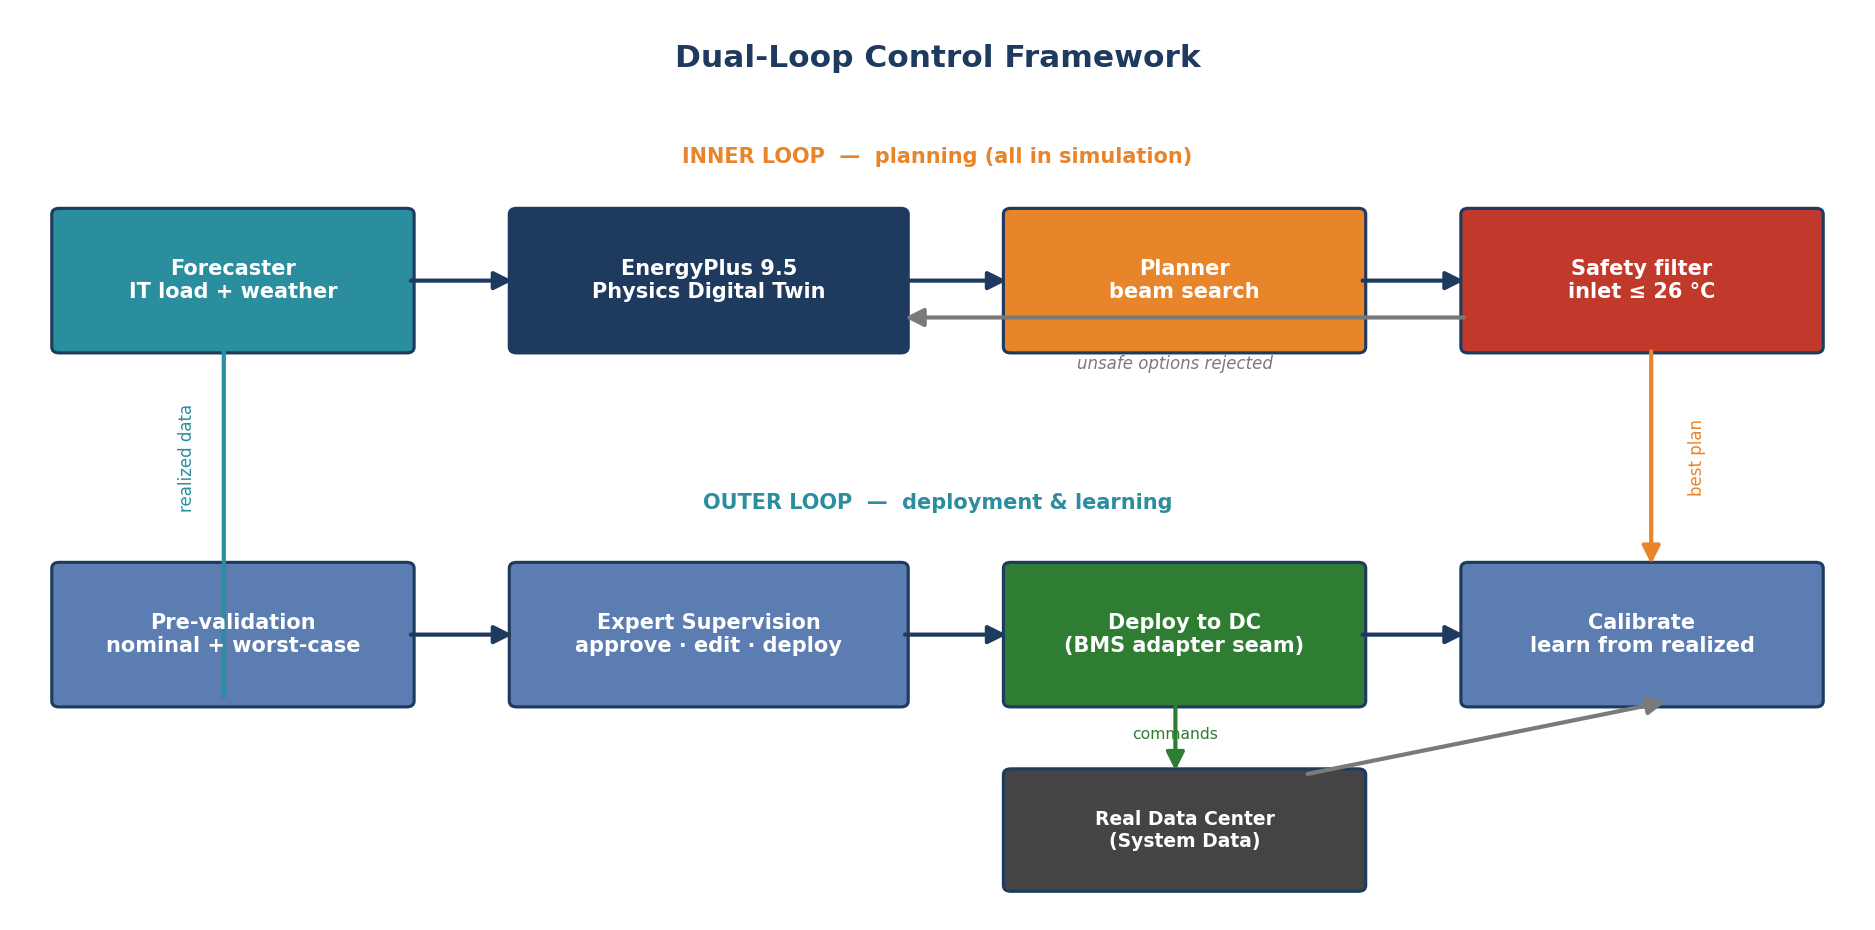
\includegraphics[width=\linewidth]{fig3_arch.png}
  \caption{The dual-loop control framework. \emph{Inner loop} (planning, all in
  simulation): forecaster \(\rightarrow\) EnergyPlus physics twin \(\rightarrow\) beam
  search \(\rightarrow\) safety filter, with unsafe candidates rejected. \emph{Outer
  loop} (deployment and learning): pre-validation \(\rightarrow\) expert supervision
  \(\rightarrow\) deploy \(\rightarrow\) calibrate from realized data, which feeds the
  forecaster and search of the next cycle.}
  \label{fig:arch}
\end{figure}

A defining property of the design is that \textbf{the same first-principles engine is the
oracle on both sides}: candidates are scored, finalists are stress-tested, and deployed
weeks are re-evaluated by the identical EnergyPlus model, so the safety argument never
leaves physics for a cheaper surrogate.

% =====================================================================
\section{Physical and Mathematical Formulation}
\label{sec:formulation}

Throughout, a week is discretized into 15-minute control steps; with the default of four
timesteps per hour, the step length is \(\Delta t = 0.25\,\mathrm{h}\). We write \(t\) for
the step index (after a warm-up discard of the first six samples), \(r\) for a server-rack
(ITE) index, and \(z\) for a thermal zone. The hard inlet cap is
\(\Tcap = 26.0\,\degC\). Table~\ref{tab:constants} (Appendix~\ref{app:notation}) collects
every constant.

\subsection{The EnergyPlus oracle and KPI aggregation}
\label{sec:oracle}
Each candidate setpoint triple is evaluated by a complete week-long EnergyPlus~9.5
simulation, run inside a Docker container and coupled to the controller through a BCVTB
socket. Because the dctwin/EnergyPlus configuration is a process-global singleton, the
oracle parallelizes \emph{across processes}, fanning candidates out over a
\code{ProcessPoolExecutor}. Each evaluation is bounded by a per-candidate watchdog
(\(300\,\mathrm{s}\)), a batch deadline, and a stall watchdog that abandons stragglers if
nothing completes within \(1.5\times\) the timeout --- so a hung container costs minutes,
not the whole plan.

From the per-step EnergyPlus output the oracle computes the controllable HVAC power. The
energy objective is \emph{hall-scoped} (scope \code{hall\_controllable\_v1}): it sums the
1F-2A ACU fan powers and the shared chiller/CHW-plant powers, rather than the cruder
``facility total minus IT.'' Writing \(\mathcal{H}\) for the set of discovered controllable
power channels (ACU fans \(\cup\) chiller/CHW plant) and \(P_{j,t}\) for channel \(j\)'s
power at step \(t\),
\begin{equation}
P^{\mathrm{hvac}}_t =
\begin{cases}
\displaystyle\sum_{j\in\mathcal{H}} P_{j,t}, & \text{if controllable channels are discovered,}\\[10pt]
P^{\mathrm{total}}_t - P^{\mathrm{IT}}_t, & \text{fallback (mock/legacy).}
\end{cases}
\label{eq:phvac}
\end{equation}
The fallback (facility power minus IT power) is used only when the component channels are
not present, e.g.\ in unit-test stand-ins. Per-step energy and the weekly total follow as
\begin{equation}
E_t = \frac{P^{\mathrm{hvac}}_t\,\Delta t}{1000}\;[\mathrm{kWh}],
\qquad
\Esum = \sum_t E_t \;[\mathrm{kWh}],
\label{eq:energy}
\end{equation}
where the factor \(1/1000\) converts \(\mathrm{W{\cdot}h}\) to \(\mathrm{kWh}\). The mean
Power Usage Effectiveness is computed facility-wide and only over steps with non-zero IT
power,
\begin{equation}
\overline{\mathrm{PUE}} = \frac{1}{\lvert\{t: P^{\mathrm{IT}}_t>0\}\rvert}
\sum_{t:\,P^{\mathrm{IT}}_t>0} \frac{P^{\mathrm{total}}_t}{P^{\mathrm{IT}}_t}.
\label{eq:pue}
\end{equation}
The safety-relevant KPIs are the peak inlet temperature, the count of hard violations,
and a soft excess accumulator,
\begin{align}
T^{\mathrm{inlet}}_{\max} &= \max_t\Big(\max_r T_{r,t}\Big), \label{eq:tmax}\\
N^{\mathrm{inlet}}_{\mathrm{viol}} &= \sum_t \mathbb{1}\!\left[\max_r T_{r,t} > \Tcap\right], \label{eq:nviol}\\
S^{\mathrm{inlet}} &= \sum_t \max\!\Big(\max_r T_{r,t} - T_{\mathrm{soft}},\,0\Big),
\quad T_{\mathrm{soft}} = \Tcap - 1.0 = 25.0\,\degC, \label{eq:sinlet}
\end{align}
where \(T_{r,t}\) is the inlet dry-bulb temperature at rack \(r\) and step \(t\). Two
further soft accumulators penalize relative-humidity excursions outside \([30\%,60\%]\)
and zone-temperature deviation from the tropical band \(32\pm1\,\degC\):
\begin{align}
S^{\mathrm{rh}} &= \sum_t\sum_h\Big[\max(\mathrm{RH}_{\min}-\mathrm{RH}_{h,t},0)
   + \max(\mathrm{RH}_{h,t}-\mathrm{RH}_{\max},0)\Big], \label{eq:srh}\\
S^{\mathrm{zone}} &= \sum_t\sum_z \max\!\Big(\lvert T^{\mathrm{zone}}_{z,t}-T^{\star}_{\mathrm{zone}}\rvert - b_{\mathrm{zone}},\,0\Big),
\label{eq:szone}
\end{align}
with \(\mathrm{RH}_{\min}=30\%\), \(\mathrm{RH}_{\max}=60\%\),
\(T^{\star}_{\mathrm{zone}}=32\,\degC\), and half-band \(b_{\mathrm{zone}}=1\,\degC\).

\subsection{Control parametrization and the broadcast map}
\label{sec:broadcast}
The decision variable is the triple \((\mathrm{SAT},\mathrm{flow},\mathrm{CHWST})\) within
the box defined above. EnergyPlus actuators are driven in a normalized
\([-1,1]\) coordinate; each physical value \(x\) with bounds \((\mathrm{lb},\mathrm{ub})\)
maps linearly as
\begin{equation}
\tilde{x} = \frac{2\,(x-\mathrm{lb})}{\mathrm{ub}-\mathrm{lb}} - 1 \in [-1,1].
\label{eq:norm}
\end{equation}
The three globals are then \emph{broadcast} to the 45-dimensional action vector by
repeating each global across its actuator group,
\begin{equation}
\underbrace{22}_{\text{SAT}} \;+\; \underbrace{22}_{\text{airflow}} \;+\; \underbrace{1}_{\text{CHWST}} \;=\; 45,
\label{eq:broadcast}
\end{equation}
each entry normalized by Eq.~\eqref{eq:norm} with its own bounds. Reducing the search to
three shared setpoints is both physically reasonable (a single hall's CRAHs are operated
in concert) and what makes a full-physics search tractable.

\subsection{The objective function}
\label{sec:objective}
Candidates are ranked by a single scalar cost that is dominated by energy and shaped by
the soft penalties. When a time-of-use tariff or grid-carbon profile is supplied, the
energy term is replaced by its hour-weighted cost,
\begin{equation}
C_{\mathrm{wgt}} = \sum_t E_t \cdot \rho\!\left[(h_0 + \lfloor t\,\Delta t\rfloor)\bmod 24\right],
\label{eq:cost}
\end{equation}
where \(\rho\) is the vector of 24 hourly rates (in \$/kWh or \(\mathrm{kgCO_2/kWh}\)) and
\(h_0\) is the hour-of-day of the first scored step. The scalar objective (lower is
better) is
\begin{equation}
J = E^{\star} + \lambda_T\,S^{\mathrm{inlet}} + \lambda_{\mathrm{rh}}\,S^{\mathrm{rh}} + \lambda_z\,S^{\mathrm{zone}},
\qquad
E^{\star} = \begin{cases} C_{\mathrm{wgt}}, & \text{tariff set,}\\ \Esum, & \text{otherwise,}\end{cases}
\label{eq:objective}
\end{equation}
with weights \(\lambda_T=1.0\) (per \(\degC{\cdot}\)step of inlet excess),
\(\lambda_{\mathrm{rh}}=0.2\), \(\lambda_z=0.1\). An infeasible candidate (next section)
is assigned \(J=+\infty\); so is any candidate whose computed cost is non-finite. Crucially,
\emph{feasibility never trades against price}: the soft penalties shape the search among
\emph{feasible} options, they cannot buy a violation. The headline operational metric is
the energy reduction against the as-operated baseline,
\begin{equation}
\Delta E_{\%} = \frac{E_{\mathrm{base}} - E_{\mathrm{plan}}}{E_{\mathrm{base}}}\times 100,
\label{eq:reduction}
\end{equation}
where \(E_{\mathrm{base}}\) is the energy of the as-operated setpoints (the historical
operating point, Section~\ref{sec:baseline}) evaluated once by the same oracle.

\subsection{Forecasting the week ahead}
\label{sec:forecaster}
Both the IT load and the weather for the coming week are forecast from history, since the
planner runs a week before the controlled period.

\paragraph{IT load.} The per-hall IT load \(L_t\) (kW) is converted to a CPU-loading
fraction against nameplate capacity \(C = \mathrm{total\_watts}/1000\) (kW),
\begin{equation}
u_t = \mathrm{clip}\!\Big(\frac{L_t}{C},\,0,\,1\Big).
\label{eq:loadfrac}
\end{equation}
A seasonal climatology is built by bucketing historical observations by weekday and
time-of-day bin, and the forecast for step \(i\) is the empirical percentile of its
bucket,
\begin{equation}
\widehat{u}^{(q)}_i = \mathrm{percentile}_q\big(\{u : \text{same (weekday, time-bin) bucket}\}\big),
\quad q\in\{10,50,90\},
\label{eq:climatology}
\end{equation}
giving p10/p50/p90 bands; the point forecast is the p50. The pooled diurnal shape is then
re-leveled to the target period by a clipped ratio of local-to-global daily means,
\begin{equation}
\kappa = \mathrm{clip}\!\Big(\frac{\mu_{\mathrm{local}}}{\mu_{\mathrm{global}}},\,0.5,\,1.5\Big),
\label{eq:level}
\end{equation}
with \(\mu_{\mathrm{local}}\) the mean of whole-day means in a \(\pm 10\)-day window around
the week start and \(\mu_{\mathrm{global}}\) the all-history mean. For this hall the IT load
is nearly flat month-to-month, so in practice \emph{weather} drives the week-to-week
variation.

\paragraph{Weather.} For the target week we compute historical-analog statistics of the
outdoor dry-bulb temperature over all years, using rows whose month-day falls within the
target week padded by \(\pm 7\) days,
\begin{equation}
\mu_c = \mathrm{mean}\big(\{T_{\mathrm{db}}\}\big),
\qquad
\sigma_c = \mathrm{pstdev}\big(\{T_{\mathrm{db}}\}\big).
\label{eq:weatherstats}
\end{equation}
From these we synthesize EnergyPlus weather-file (EPW) variants by shifting the entire
dry-bulb series,
\begin{equation}
\delta = k\,\sigma_c,
\qquad
\{\text{nominal}: 0,\ \text{hot}: +\delta,\ \text{cool}: -\delta\},
\quad k=1,
\label{eq:weathervariants}
\end{equation}
with the dew point clamped not to exceed the shifted dry-bulb. The \(+1\sigma\) ``hot''
variant is added as an extra scenario in the robustness gate (Section~\ref{sec:safety}),
so the plan must hold the inlet cap even in an unusually hot week.

\subsection{The recirculation fidelity model}
\label{sec:recirc}
The link between a CRAH's supply-air temperature and a server's \emph{inlet} temperature is
not the identity: in any real hall some fraction of hot exhaust air recirculates into the
cold aisle. We model this with the standard mixing identity --- the inlet is a blend of
supply and return air,
\begin{equation}
T_{\mathrm{inlet}} = r\,T_{\mathrm{return}} + (1-r)\,T_{\mathrm{supply}}
\quad\Longrightarrow\quad
r = \frac{T_{\mathrm{inlet}} - T_{\mathrm{supply}}}{T_{\mathrm{return}} - T_{\mathrm{supply}}},
\label{eq:mixing}
\end{equation}
where \(r\in[0,1]\) is the recirculation fraction. Given measured rack temperatures the
fraction is estimated robustly as a clipped median, discarding steps whose supply/return
gap is too small to be informative (\(<1\,\degC\)):
\begin{equation}
\widehat{r} = \mathrm{median}\Big\{\mathrm{clip}(r,\,0,\,R_{\max}) :
\lvert T_{\mathrm{return}} - T_{\mathrm{supply}}\rvert \ge 1\,\degC\Big\},
\qquad R_{\max}=0.5.
\label{eq:rhat}
\end{equation}
Recirculation worsens when CRAH airflow undershoots the IT demand, so we add a
flow-shortfall term to the calibrated baseline fraction \(r_0\),
\begin{equation}
r_{\mathrm{eff}} = \min\!\Big(R_{\max},\; r_0 + k_r\,\max\!\big(0,\ 1 - \tfrac{\mathrm{flow}}{\mathrm{demand}}\big)\Big),
\qquad k_r=0.5,
\label{eq:reff}
\end{equation}
and apply a \emph{conservative-only} (safety-tightening) correction to the predicted
inlet,
\begin{equation}
T'_{\mathrm{inlet}} = T_{\mathrm{inlet}} + \max\!\Big(0,\ (r_{\mathrm{eff}}-r_0)\,\max(0,\ T_{\mathrm{zone}} - T_{\mathrm{inlet}})\Big).
\label{eq:recirccorr}
\end{equation}
When the airflow meets demand, \(r_{\mathrm{eff}}=r_0\) and the correction is exactly zero;
the model can only raise the inlet, never lower it. Until calibrated against real rack
sensors the correction defaults to a provable no-op, so no inlet margin is invented.

% =====================================================================
\section{Optimization: Coarse-to-Fine Beam Search}
\label{sec:search}

The inner loop searches the three-dimensional setpoint box with a best-first beam search
that refines a coarse grid. At level~0 it evaluates a regular grid,
\begin{equation}
\mathrm{grid} = \mathrm{linspace}(\mathrm{lb},\mathrm{ub},g)^{\otimes 3},
\qquad g=5 \;\Rightarrow\; 5^3 = 125 \text{ candidates},
\label{eq:grid}
\end{equation}
keeps the top-\(B\) (beam width \(B=5\)) by score, and refines each survivor by exploring a
neighborhood whose step is half the coarse spacing and halves again every level,
\begin{equation}
\Delta^{(0)}_d = \frac{\mathrm{ub}_d-\mathrm{lb}_d}{2(g-1)},
\qquad
\Delta^{(\ell+1)}_d = \tfrac{1}{2}\,\Delta^{(\ell)}_d,
\qquad d\in\{\mathrm{SAT},\mathrm{flow},\mathrm{CHWST}\}.
\label{eq:refstep}
\end{equation}
Each candidate's neighbors are axis and pairwise-diagonal offsets clipped to the box; the
beam is re-selected by a stable ascending sort on \(J\) (infeasible candidates, scored
\(+\infty\), sink to the bottom). Refinement stops early when the best score stops
improving,
\begin{equation}
\big\lvert J^{(\ell-1)}_{\mathrm{best}} - J^{(\ell)}_{\mathrm{best}}\big\rvert
< \epsilon\,\max\!\big(\lvert J^{(\ell-1)}_{\mathrm{best}}\rvert,\,1\big),
\qquad \epsilon = 10^{-3}.
\label{eq:earlystop}
\end{equation}
With the default three levels this evaluates a few hundred full-week simulations per plan.
An optional time-block extension splits the week into day \([6,18)\) and night blocks and
warm-starts a coordinate-descent refinement (initial step a quarter of the range, halving
per level) from the constant-setpoint optimum, allowing distinct day/night setpoints when
they help.

\paragraph{Degenerate-signal guard.} A physics model wired incorrectly can be
\emph{control-invariant} --- every setpoint yields the same energy and inlet, so the search
optimizes noise. The optimizer therefore flags a degenerate level when both the inlet and
energy spreads collapse,
\begin{equation}
\Big(\max_i T^{\mathrm{inlet}}_{\max,i} - \min_i T^{\mathrm{inlet}}_{\max,i}\Big) < 0.1\,\degC
\quad\wedge\quad
\frac{\max_i E_i - \min_i E_i}{\overline{E}} < 0.01 .
\label{eq:degen}
\end{equation}

\paragraph{The optimization is physically well-posed.} A direct EnergyPlus sweep
(Fig.~\ref{fig:wellposed}) confirms that the three setpoints exert a real, well-separated
physical gradient on energy while the inlet cap binds: across its range \emph{airflow}
moves hall cooling energy by \(15.5\%\), \emph{CHWST} by \(3.4\%\), and \emph{SAT} by
\(\approx 0.5\%\). The cheapest operating point (lowest airflow) is also the one that runs
the inlet closest to the cap, which is exactly why a search with a hard constraint --- not
an unconstrained minimization --- is required.

\begin{figure}[t]
  \centering
  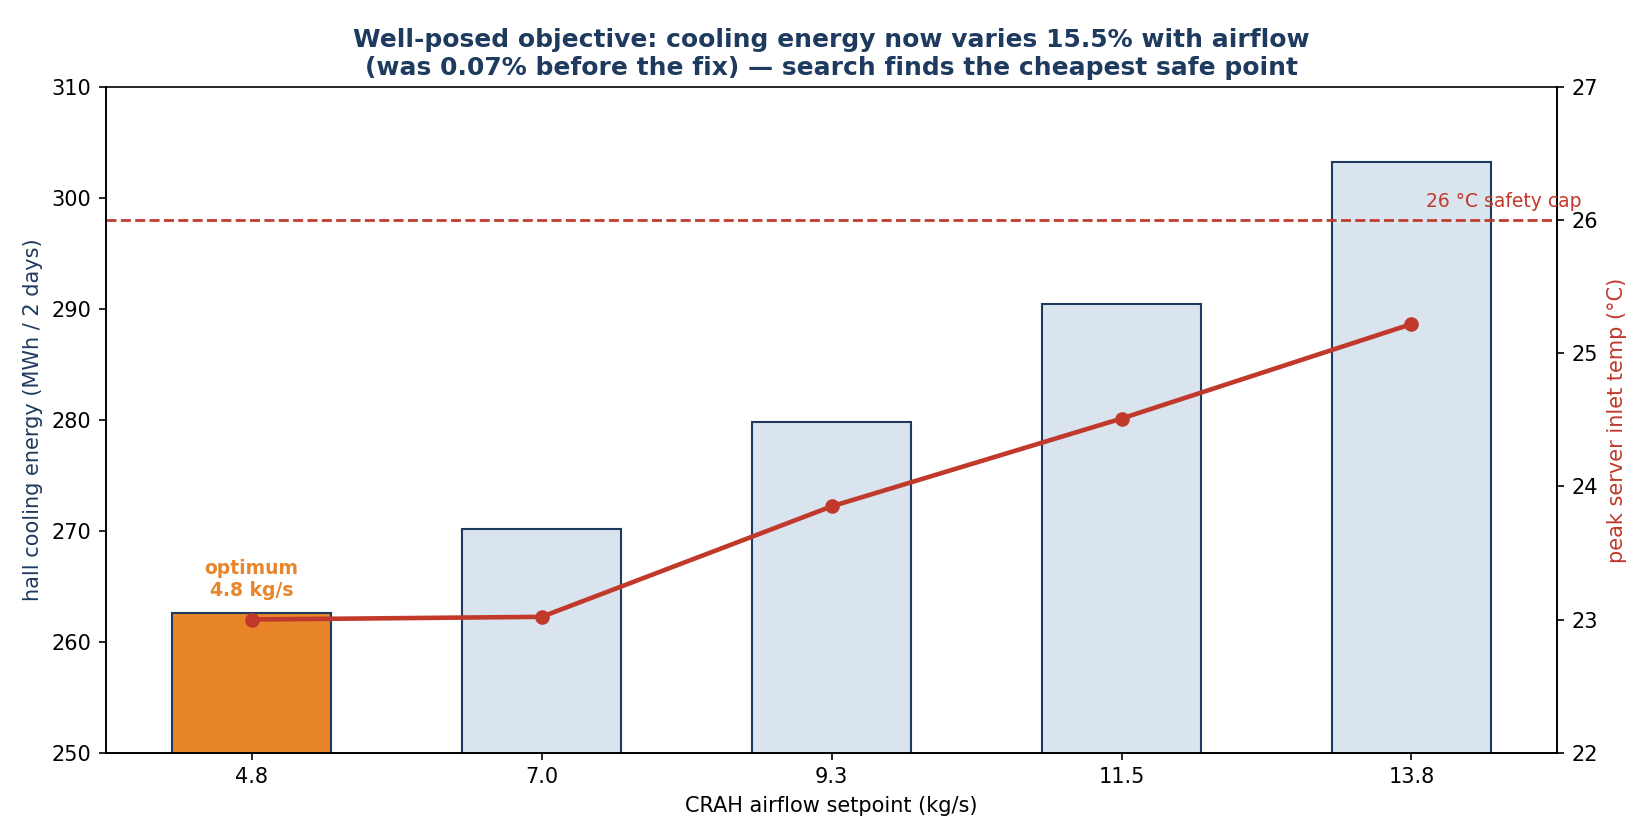
\includegraphics[width=0.86\linewidth]{fig4_results.png}
  \caption{Well-posedness sweep (real EnergyPlus). Bars: hall cooling energy versus CRAH
  airflow; line: peak server inlet versus airflow, against the \(26\,\degC\) cap. Cooling
  energy varies \(15.5\%\) across the airflow range (\(3.4\%\) for CHWST, \(\approx0.5\%\)
  for SAT) --- a true physical gradient --- while the cheapest (lowest-airflow) point is the
  hottest, so the constrained search is meaningful.}
  \label{fig:wellposed}
\end{figure}

% =====================================================================
\section{Safety: The Three-Net Robust Gate}
\label{sec:safety}

Safety is enforced by three independent nets (Fig.~\ref{fig:safety}), each strictly
necessary, with model uncertainty hedged exactly once.

\subsection{Net 1 --- hard cap with a \texorpdfstring{$k\sigma$}{k-sigma} margin}
A candidate is \emph{feasible} only if it satisfies all of:
\begin{equation}
\text{feasible} \;\wedge\;
\big(N^{\mathrm{inlet}}_{\mathrm{viol}} \le 0\big) \;\wedge\;
\big(m_{\mathrm{fc}}=0 \ \lor\ T^{\mathrm{inlet}}_{\max}+m_{\mathrm{fc}} \le \Tcap\big),
\label{eq:feasible}
\end{equation}
i.e.\ \emph{zero} steps above the cap, and the peak inlet at least a margin
\(m_{\mathrm{fc}}\) below it. The margin pre-tightens the cap by \(k_\sigma\) standard
deviations of the twin's inlet-prediction error,
\begin{equation}
m_{\mathrm{fc}} = k_\sigma\,\sigma_{\mathrm{inlet}},
\qquad k_\sigma = 1.0,
\qquad
\sigma_{\mathrm{inlet}} =
\begin{cases}
\sigma^{\mathrm{floor}}_{\mathrm{inlet}}, & n_{\mathrm{weeks}}>0,\\[3pt]
1.0\,\degC, & n_{\mathrm{weeks}}=0 \ (\text{cold start}),
\end{cases}
\label{eq:margin}
\end{equation}
where \(\sigma^{\mathrm{floor}}\) is the fading-floor calibration uncertainty
(Section~\ref{sec:calib}). At cold start the effective cap is \(26-1.0 = 25.0\,\degC\); as
weeks accumulate and the twin earns confidence, \(\sigma_{\mathrm{inlet}}\) shrinks and
more of the \(26\,\degC\) headroom becomes usable.

\subsection{Net 2 --- a data-centered robust ensemble}
The few finalists from the search are re-simulated on an \emph{ensemble} of perturbed
plants, plus the \(+1\sigma\) hot-weather week of Eq.~\eqref{eq:weathervariants}. The
ensemble is centered on the \emph{believed} plant (the data-driven plant parameters fitted
by recalibration, Section~\ref{sec:recalib}; a fixed default until then), and its width is
set by the posterior uncertainty. Scenario \(i\) scales each plant perturbation factor by
\begin{equation}
m_i = (1-s) + 2s\cdot\frac{i}{n-1},\qquad i=0,\dots,n-1,
\label{eq:multipliers}
\end{equation}
where the half-width \(s\) adapts to measured confidence,
\begin{equation}
s = \min\!\Big(s_{\mathrm{base}},\ \max\!\big(s_{\min},\ s_{\mathrm{base}}\cdot \tfrac{\sigma_{\mathrm{post,inlet}}}{\sigma_{\mathrm{ref}}}\big)\Big),
\qquad s_{\mathrm{base}}=0.10,\ s_{\min}=0.02,\ \sigma_{\mathrm{ref}}=1.0,
\label{eq:halfwidth}
\end{equation}
so the spread never falls below a \(\pm 2\%\) physical-drift floor and never exceeds the
\(\pm 10\%\) cold-start bracket. Inside these scenarios the \(k\sigma\) margin is switched
\emph{off} (\(m_{\mathrm{fc}}=0\)): the uncertainty is spent once, in the ensemble width,
not double-counted against a margin as well. Across the scenario KPIs the gate summarizes
the energy tail with the conditional value-at-risk and reports robust bands by quantiles,
\begin{equation}
\mathrm{CVaR}_\alpha(\{v_i\}) = \frac{1}{k}\sum_{j=1}^{k} v^{\downarrow}_{(j)},
\qquad k = \max\!\big(1, \lceil (1-\alpha) N\rceil\big),
\qquad \alpha = 0.8,
\label{eq:cvar}
\end{equation}
with \(v^{\downarrow}\) the energies sorted worst-first. A finalist is \textbf{robustly
feasible} iff a majority of its scenarios complete and \emph{every} completed scenario is
feasible by Eq.~\eqref{eq:feasible} (with scenario KPIs bias-corrected and tested against
the hard cap):
\begin{equation}
\lvert\mathcal{K}_i\rvert \ge \Big\lceil \tfrac{n_{\mathrm{req}}}{2}\Big\rceil
\quad\wedge\quad
\forall k\in\mathcal{K}_i:\ \mathrm{is\_feasible}(k).
\label{eq:robustfeas}
\end{equation}
The winner is the robustly feasible finalist of least energy CVaR.

\paragraph{The safety ladder.} If the energy optimum is \emph{fragile} --- cheap on the
nominal plant but not robustly feasible --- the gate does not simply block. It walks a
\emph{safety ladder} from the chosen point toward the guaranteed-safe corner
\((\mathrm{SAT},\mathrm{flow},\mathrm{CHWST}) = (20.0,\,13.8,\,13.0)\), spending the
\emph{cheapest} axis first. Because CHWST moves energy only \(\approx 3\%\) while airflow
moves it \(\approx 15\%\) (Section~\ref{sec:search}), the ladder lowers chilled-water
temperature before it raises airflow, substituting the least-costly provably-robust plan
rather than returning nothing actionable.

\subsection{Net 3 --- the deploy backstop}
After a week is realized, any single inlet violation marks the plan \code{deploy\_blocked}
rather than \code{deployed}. This zero-tolerance backstop closes the loop: a plan that
slipped through prediction is never recorded as a clean deployment.

\begin{figure}[t]
  \centering
  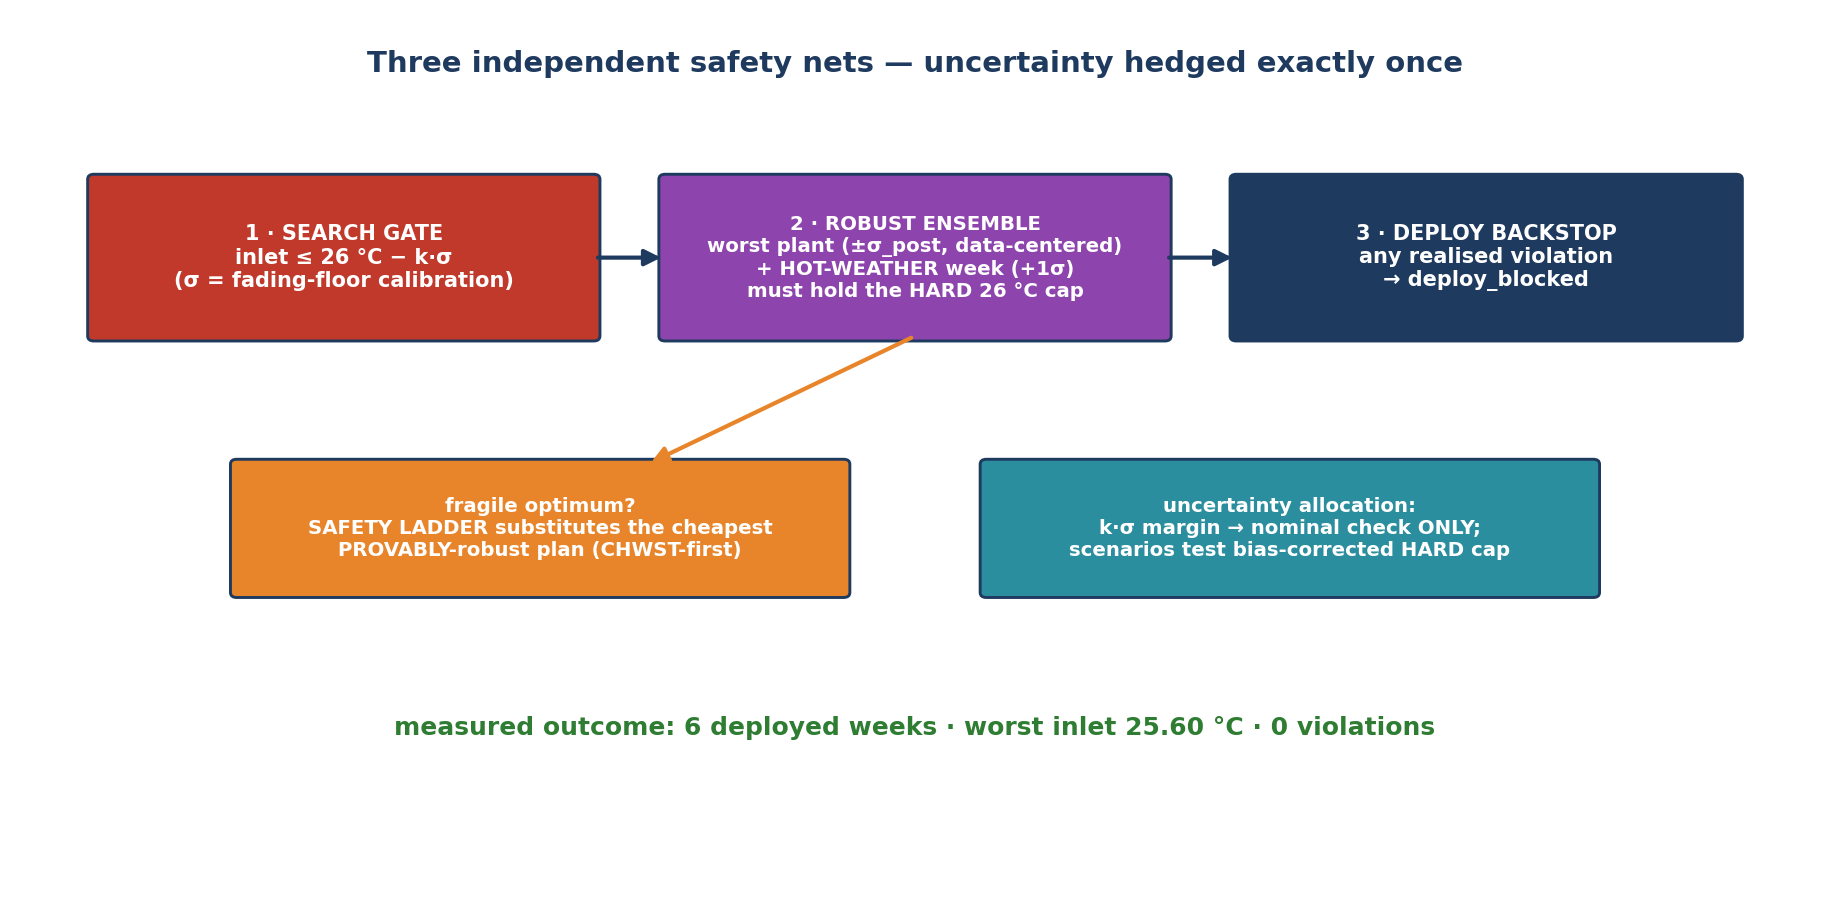
\includegraphics[width=\linewidth]{figD_safety_stack.png}
  \caption{The three-net safety architecture. Net~1: the hard \(26\,\degC\) cap pre-tightened
  by a \(k\sigma\) margin in the search. Net~2: a data-centered worst-case ensemble
  (plant \(\pm\sigpost\) plus a \(+1\sigma\) hot-weather week) that must hold the
  \emph{hard} cap, with uncertainty spent exactly once and a safety ladder substituting the
  cheapest provably-robust plan for a fragile optimum. Net~3: a zero-tolerance deploy
  backstop. Measured outcome over six deployed weeks: worst inlet \(25.60\,\degC\), zero
  violations.}
  \label{fig:safety}
\end{figure}

% =====================================================================
\section{The Outer Loop: Learning from Reality}
\label{sec:outer}

The twin improves itself on two timescales: a fast \emph{output} calibration after every
deployed week, and a slow \emph{parameter} recalibration once a bias persists.

\subsection{Output calibration: bias and two uncertainties}
\label{sec:calib}
After each deployed week the paired (predicted \(p\), realized \(r\)) values of three KPIs
--- weekly HVAC energy, mean PUE, and peak inlet --- update the calibration state. Residuals
are winsorized to a per-KPI clip \(c\) to keep one anomalous week from poisoning the
estimate, and the bias is their mean,
\begin{equation}
e_w = \mathrm{clip}(r-p,\,-c,\,+c),
\qquad
b = \frac{1}{n}\sum_{w=1}^{n} e_w,
\label{eq:bias}
\end{equation}
with \(n\) the number of paired weeks. Two uncertainties are maintained from the same
residuals. The \emph{fading-floor} \(\sigma\), which backs the \(k\sigma\) search margin of
Eq.~\eqref{eq:margin}, never understates early because it is floored by a decaying prior,
\begin{equation}
\sigma^{\mathrm{floor}} = \max\!\Big(s,\ \frac{\sigma_{\mathrm{prior}}}{n}\Big),
\qquad
s = \sqrt{\frac{1}{n}\sum_{w=1}^{n}(e_w-b)^2},
\label{eq:fadingfloor}
\end{equation}
so that at \(n=1\) (where the sample std \(s=0\)) the uncertainty equals the prior rather
than a dangerous zero, and the floor \(\sigma_{\mathrm{prior}}/n\) decays as evidence
accumulates. The \emph{empirical-Bayes posterior} \(\sigma\), which sizes the robust
ensemble of Eq.~\eqref{eq:halfwidth}, blends the sample variance with the prior as if the
prior were one pseudo-week~\cite{casella},
\begin{equation}
\sigpost = \sqrt{\frac{n\,s^2 + \sigma_{\mathrm{prior}}^2}{n+1}}.
\label{eq:sigpost}
\end{equation}
It tends to \(\sigma_{\mathrm{prior}}\) at \(n=0\) and to \(s\) as \(n\to\infty\). The
inlet priors are \(\sigma_{\mathrm{prior}}=1.0\,\degC\) for the fading floor. Finally, the
learned bias is applied to future predictions, and --- because a bias added to a peak cannot
reconstruct per-step counts --- if a bias-corrected peak inlet would exceed the cap, the
violation count is forced to at least one so the feasibility gate rejects it:
\begin{equation}
x'_{\mathrm{field}} = x_{\mathrm{field}} + b_{\mathrm{field}};
\qquad
\text{if } T^{\mathrm{inlet}}_{\max}+b > 26.0:\ N^{\mathrm{inlet}}_{\mathrm{viol}}\leftarrow \max(N^{\mathrm{inlet}}_{\mathrm{viol}},1).
\label{eq:biasapply}
\end{equation}

\subsection{Physics recalibration: learning the plant's parameters}
\label{sec:recalib}
Output calibration corrects the twin's \emph{predictions}; physics recalibration corrects
the twin's \emph{model}. Once at least four weeks show a persistent energy bias, the system
fits a bounded fan-efficiency correction. The per-week realized/predicted energy ratio is
winsorized and averaged to a persistent bias fraction,
\begin{equation}
\varrho_i = \mathrm{clip}\!\Big(\frac{r_i}{p_i},\,0.5,\,2.0\Big),
\qquad
b = \frac{1}{m}\sum_{i=1}^{m}\varrho_i - 1,
\label{eq:ratio}
\end{equation}
and converted to a multiplicative correction on the EnergyPlus fan total efficiency,
\begin{equation}
\phi = \mathrm{clip}\!\Big(\frac{1}{1+b},\,0.85,\,1.15\Big),
\label{eq:phi}
\end{equation}
clamped never to propose more than a \(\pm15\%\) efficiency change, and emitted only when
\(m\ge 4\) and \(\lvert b\rvert \ge 0.01\). More realized energy than predicted
(\(b>0\)) yields \(\phi<1\) --- the fans were modeled as too efficient. The fitted factor is
persisted to the plant-calibration file and \emph{becomes the center of the robust
ensemble} (Section~\ref{sec:safety}): the twin's plant parameters now learn, not just its
outputs.

\begin{figure}[t]
  \centering
  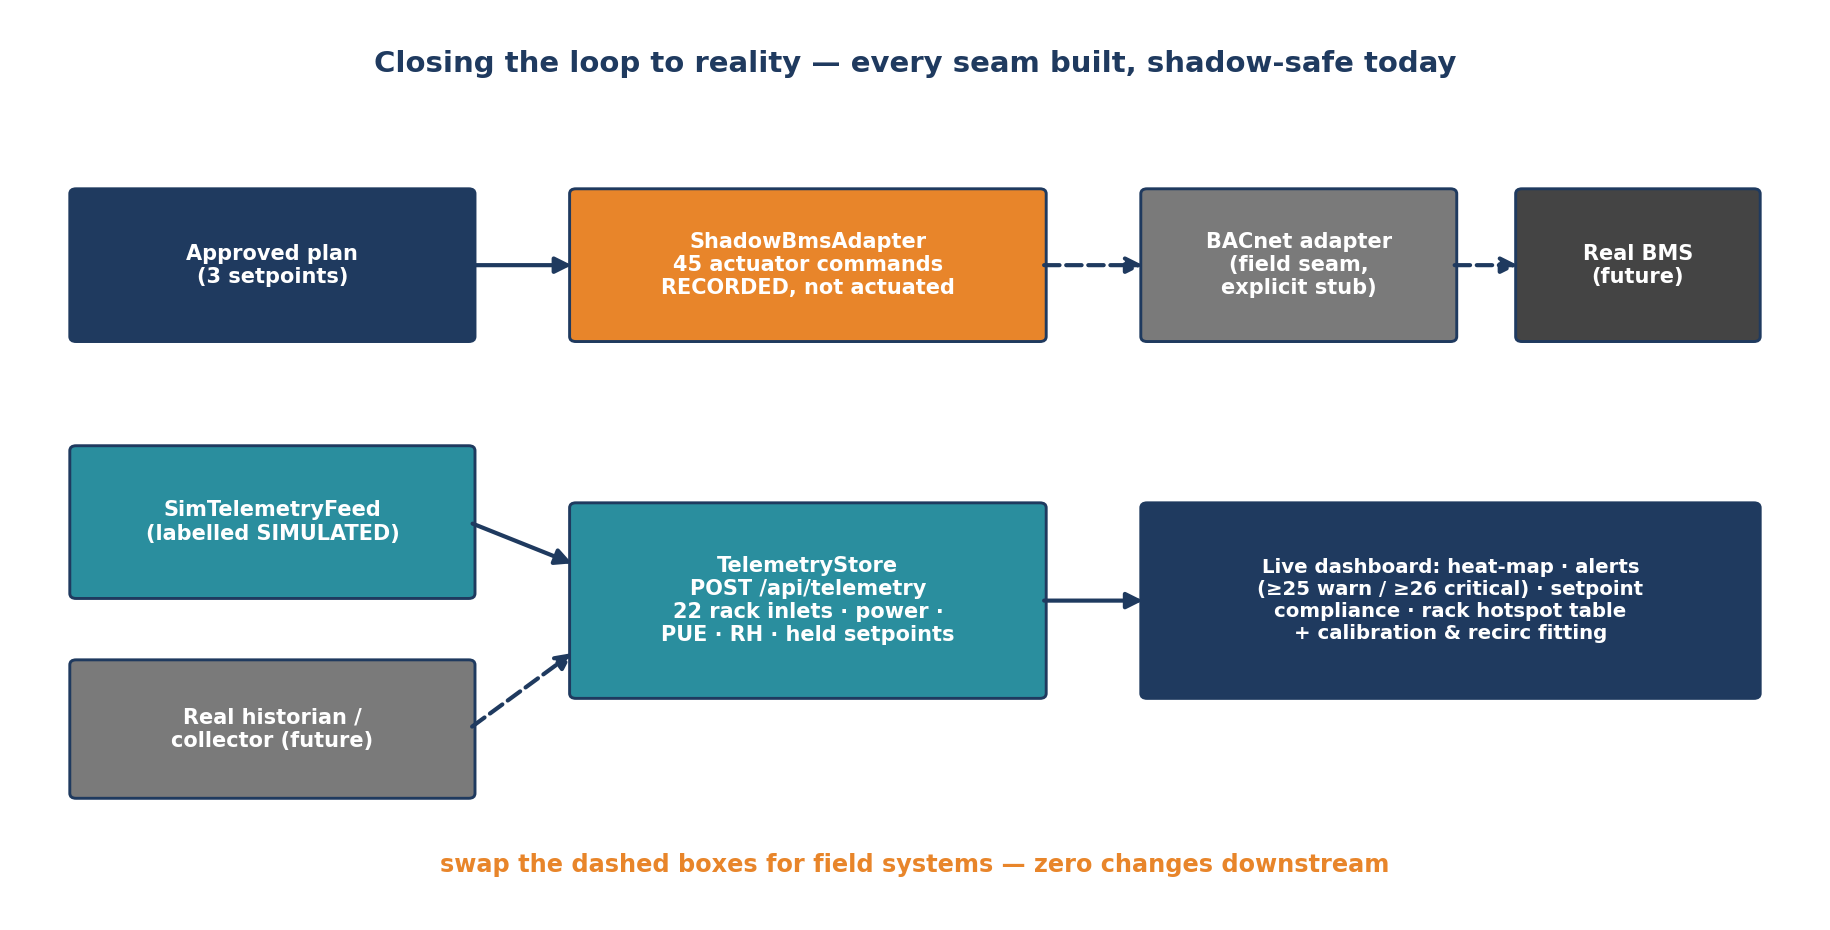
\includegraphics[width=\linewidth]{figE_dataflow.png}
  \caption{Closing the loop to reality. An approved plan becomes 45 actuator commands
  written by a shadow BMS adapter (recorded, not actuated); a telemetry store accepts any
  historian push (\code{POST /api/telemetry}) and feeds the live dashboard, calibration,
  and recirculation fitting. The dashed boxes --- a real historian collector and a BACnet
  field adapter --- are the only unbuilt seams; everything downstream is unchanged when they
  are connected.}
  \label{fig:dataflow}
\end{figure}

\subsection{The as-operated baseline}
\label{sec:baseline}
Savings are reported against the \emph{as-operated} baseline --- the operator's own
historical setpoints --- not against an artificial worst case. Baseline SAT and CHWST are
the pooled medians of the corresponding telemetry columns, and baseline airflow is derived
from the median fan speed scaled to design flow,
\begin{equation}
\mathrm{SAT}_{\mathrm{base}} = \mathrm{clip}\big(\widetilde{\mathrm{SAT}}\big),\quad
\mathrm{CHWST}_{\mathrm{base}} = \mathrm{clip}\big(\widetilde{\mathrm{CHWST}}\big),\quad
\mathrm{flow}_{\mathrm{base}} = \mathrm{clip}\!\Big(\tfrac{\widetilde{\mathrm{fan\_speed}}}{\mathrm{fan\_speed}_{\max}}\,\dot m_{\mathrm{design}}\Big),
\label{eq:baseline}
\end{equation}
where \(\widetilde{(\cdot)}\) denotes the pooled median over matching telemetry columns and a
missing signal falls back to the axis mid-range. The baseline is evaluated once by the same
oracle and supplies \(E_{\mathrm{base}}\) in Eq.~\eqref{eq:reduction}.

% =====================================================================
\section{Web Application and Operator Workflow}
\label{sec:webapp}

The framework is delivered as a single-origin web application (a FastAPI backend serving a
React front end) so that an operator drives the loop without touching code. The backend
exposes 21 endpoints, including a server-sent-events stream for live search progress and a
telemetry push endpoint; the front end comprises seven pages. We highlight three.

The \textbf{Dashboard} (Fig.~\ref{fig:dashboard}) shows the active plan's setpoints and its
predicted KPIs against the baseline --- weekly energy, PUE, peak inlet, violation count, and
percentage reduction --- so the value and the safety margin of a recommendation are visible
at a glance. The \textbf{Live Telemetry} page (Fig.~\ref{fig:live}) renders a 22-rack inlet
heat-map, an alert banner (warn at \(\ge25\,\degC\), critical at \(\ge26\,\degC\)), a ranked
hotspot table, hall KPI tiles, and a commanded-versus-held setpoint-compliance panel that
flags any axis drifting more than \(0.5\) from the deployed command; a prominent
\textsc{Simulated Feed} badge marks the data source honestly. The \textbf{Digital Twin (3D)}
page (Fig.~\ref{fig:twin3d}) colors the hall's rack rows live from telemetry, with a heads-up
display of the active plan's setpoints and KPIs, giving immediate spatial hotspot visibility.

\begin{figure}[t]
  \centering
  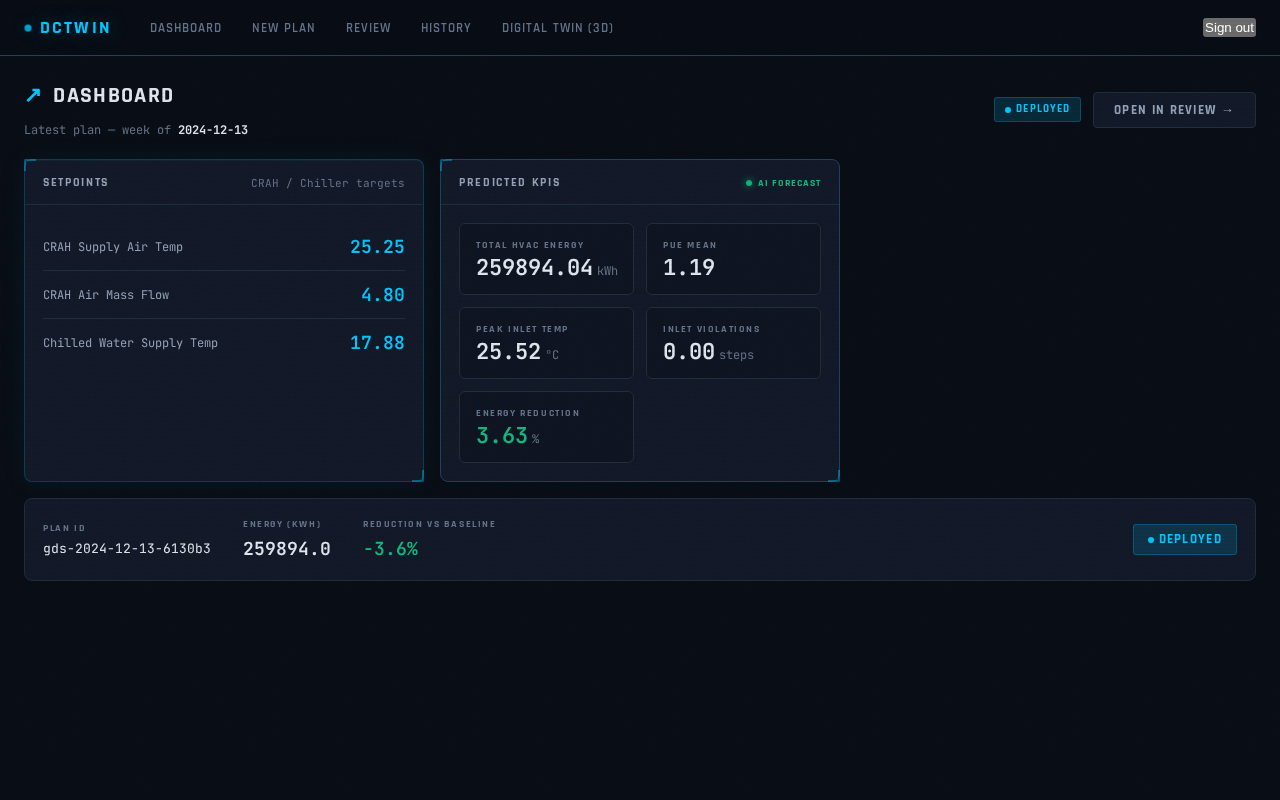
\includegraphics[width=0.92\linewidth]{shot_dashboard.png}
  \caption{Dashboard (webapp screenshot). The active plan's three setpoints (left) and its
  predicted KPIs against the as-operated baseline: weekly HVAC energy, PUE, peak inlet, and
  violations, with the energy reduction. For the displayed week the plan predicts a peak
  inlet of \(25.52\,\degC\) (below the \(26\,\degC\) cap), zero violations, and a
  \(3.63\%\) energy reduction.}
  \label{fig:dashboard}
\end{figure}

\begin{figure}[t]
  \centering
  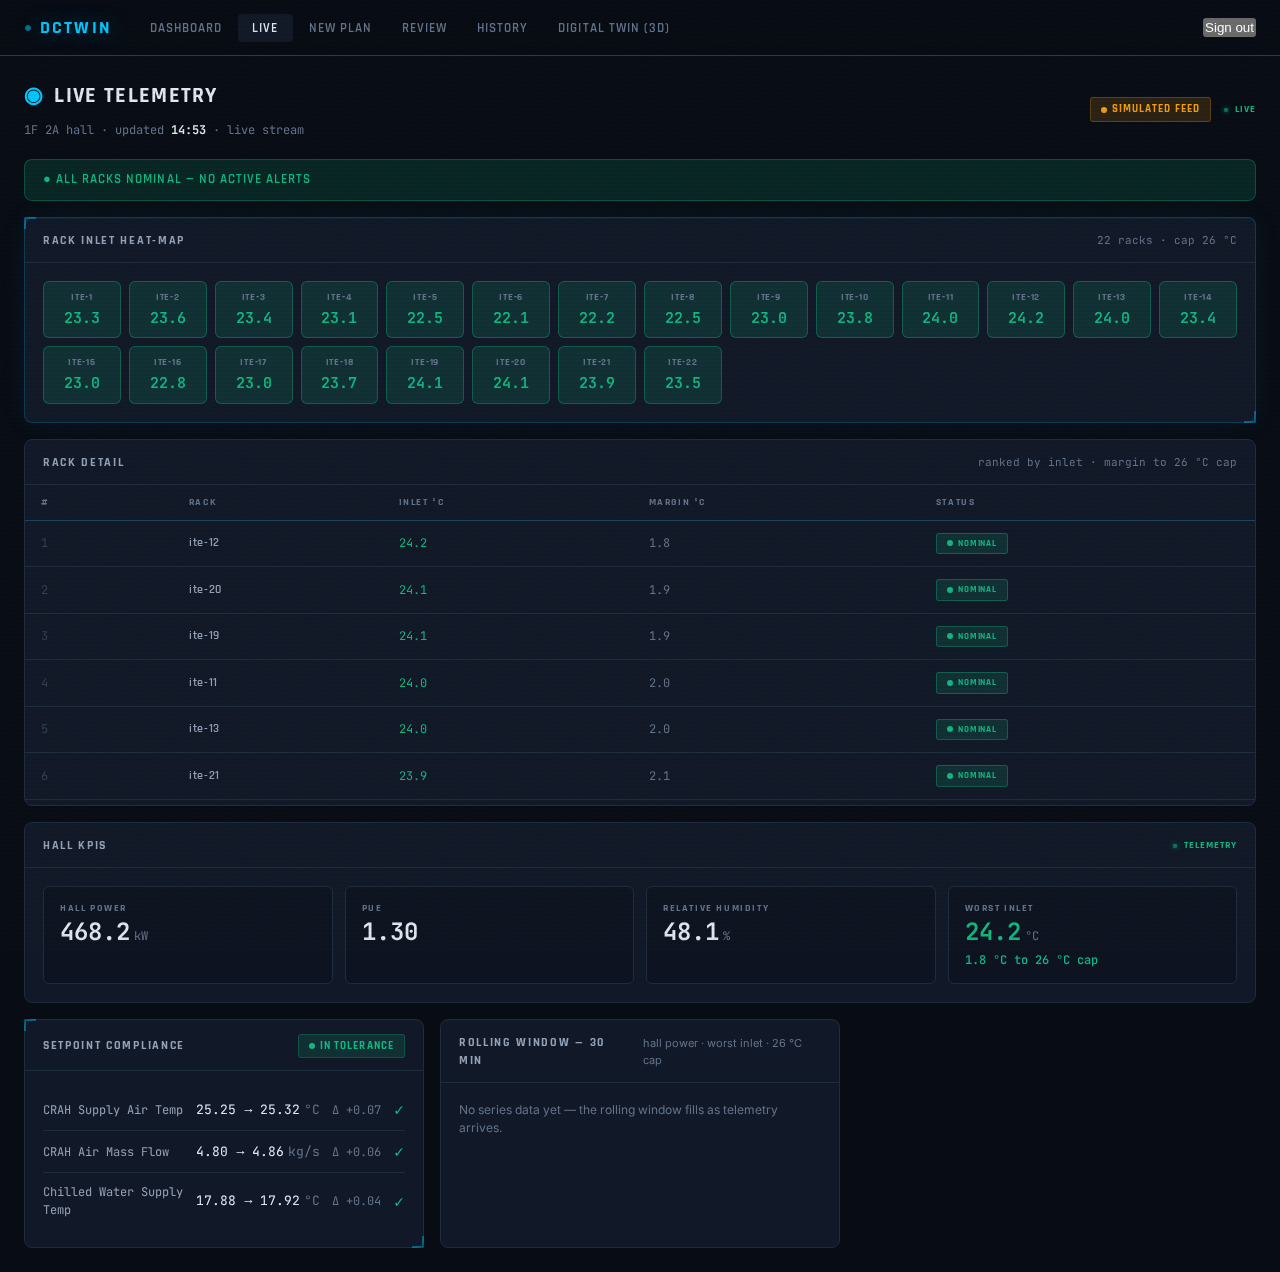
\includegraphics[width=0.78\linewidth]{shot_live.png}
  \caption{Live Telemetry (webapp screenshot). A 22-rack inlet heat-map (all green,
  \(<26\,\degC\)), the \textsc{Simulated Feed} badge, a per-rack hotspot detail table, hall
  KPI tiles (PUE, peak inlet, etc.), and the commanded-versus-held setpoint-compliance panel.
  Alerts warn at \(\ge25\,\degC\) and turn critical at \(\ge26\,\degC\).}
  \label{fig:live}
\end{figure}

\begin{figure}[t]
  \centering
  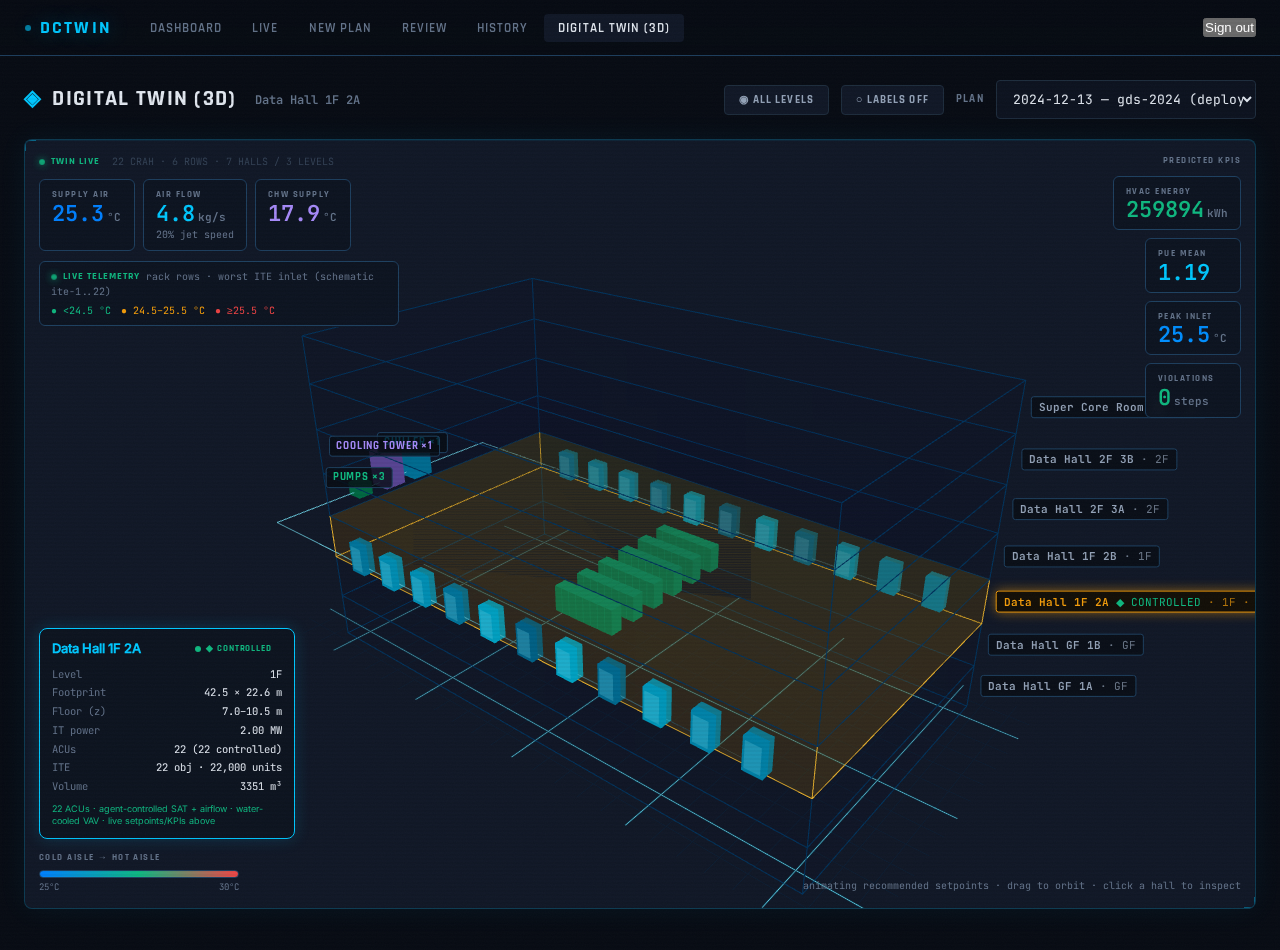
\includegraphics[width=0.92\linewidth]{shot_twin3d.png}
  \caption{Digital Twin 3D (webapp screenshot). The controlled hall's rack rows colored from
  live telemetry, with a heads-up display of the active plan's setpoints (SAT, airflow,
  CHWST) and KPIs. Spatial coloring makes any emerging hotspot immediately visible.}
  \label{fig:twin3d}
\end{figure}

The operator's weekly cycle (Fig.~\ref{fig:procedure}) is a single turn of the dual loop:
\emph{monitor} the live hall, \emph{plan} the coming week (reviewing the planning-context
decks of forecast load and weather), \emph{review} the recommendation's KPIs and inlet
trajectory against the \(26\,\degC\) line, \emph{approve} as an expert (a
\code{blocked\_unsafe} plan cannot be force-approved --- the gate refusing is the system
working), \emph{deploy} in shadow mode (45 commands recorded), and \emph{learn} as the
realized week tightens \(\sigma\) and unlocks more savings next time.

\begin{figure}[t]
  \centering
  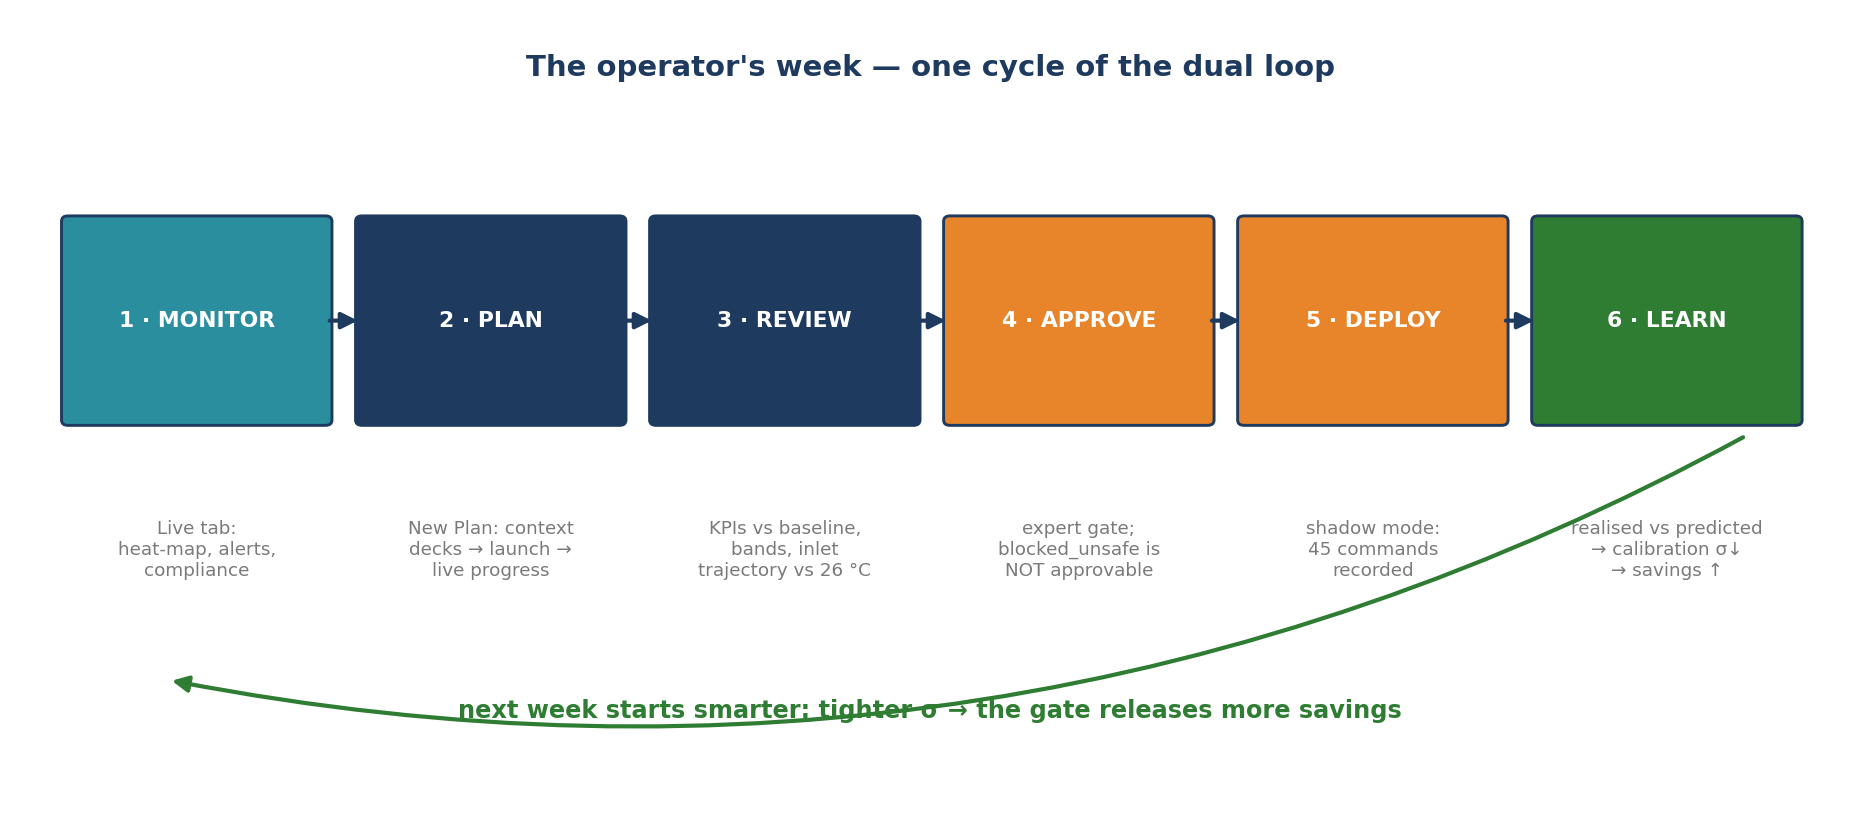
\includegraphics[width=\linewidth]{figF_procedure.png}
  \caption{The operator's week --- one cycle of the dual loop: monitor \(\rightarrow\) plan
  \(\rightarrow\) review \(\rightarrow\) approve \(\rightarrow\) shadow deploy \(\rightarrow\)
  learn. Each cycle measures the realized week, tightens the calibration uncertainty, and
  lets the safety gate release a little more saving.}
  \label{fig:procedure}
\end{figure}

% =====================================================================
\section{Experimental Results}
\label{sec:results}

We ran six consecutive weekly cycles --- plan, gate, expert-approve, (shadow) deploy,
measure, and learn --- covering the weeks beginning 2024-11-08 through 2024-12-13. All
numbers below are read from the live system's run database and calibration history;
deployment is in shadow mode, so the ``realized'' week is the same EnergyPlus model run on
a perturbed (believed) plant standing in for the field until a real telemetry collector and
BACnet adapter are connected (Section~\ref{sec:discussion}). Table~\ref{tab:weeks} reports
the per-week record.

\begin{table}[t]
\centering
\caption{Six consecutive deployed weeks. Predicted and realized weekly hall cooling energy,
absolute prediction error, energy saving versus the as-operated baseline, realized peak
server inlet, and hard-cap violations. Energy and inlet are read from the calibration
history; savings from the run database.}
\label{tab:weeks}
\small
\begin{tabular}{l r r c c c c}
\toprule
Week (start) & Pred.\ energy & Real.\ energy & \(\lvert\)Err\(\rvert\) & Saving & Peak inlet & Viol. \\
 & (kWh) & (kWh) & (\%) & (\%) & (\degC) & \\
\midrule
2024-11-08 & 273\,565 & 269\,979 & 1.33 & 0.00 & 23.37 & 0 \\
2024-11-15 & 261\,806 & 259\,583 & 0.86 & 3.20 & 24.64 & 0 \\
2024-11-22 & 260\,480 & 259\,929 & 0.21 & 3.23 & 24.68 & 0 \\
2024-11-29 & 256\,880 & 257\,368 & 0.19 & 3.60 & 25.22 & 0 \\
2024-12-06 & 258\,531 & 258\,739 & 0.08 & 3.64 & 25.57 & 0 \\
2024-12-13 & 259\,337 & 259\,603 & 0.10 & 3.63 & 25.60 & 0 \\
\bottomrule
\end{tabular}
\end{table}

\paragraph{The twin predicts reality (Fig.~\ref{fig:accuracy}).} The weekly-energy
prediction error fell from \(1.33\%\) in week~1 to \(0.10\%\) by week~6, as the output
calibration of Section~\ref{sec:calib} learned the twin's residual bias. The
safety-critical variable was predicted even better: the peak-inlet prediction error stayed
within \(0.25\,\degC\) every week, with the calibrator settling on a small positive inlet
bias (\(\approx0.18\,\degC\): the twin slightly \emph{under}-predicts the hottest inlet,
which the bias correction then adds back --- a conservative direction for safety).

\begin{figure}[t]
  \centering
  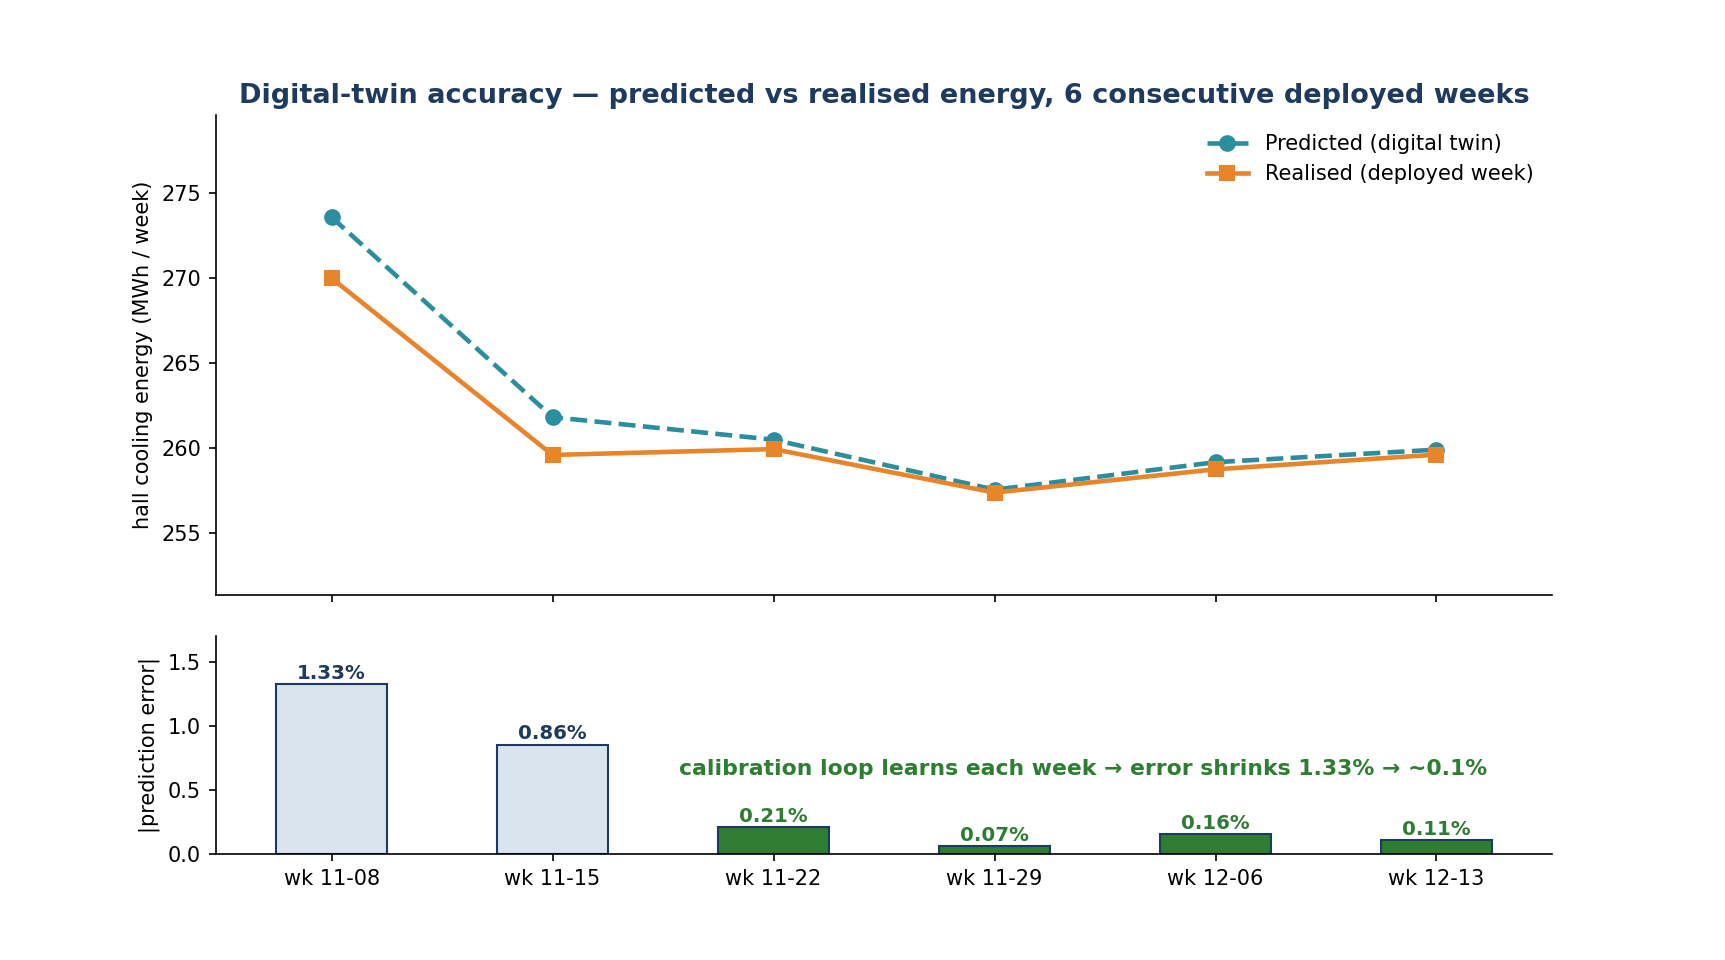
\includegraphics[width=\linewidth]{figA_accuracy.png}
  \caption{Digital-twin accuracy. Top: predicted versus realized weekly hall cooling energy
  over the six deployed weeks. Bottom: the absolute per-week prediction error, falling from
  \(1.33\%\) to \(\approx0.1\%\) as the residual-calibration loop learns.}
  \label{fig:accuracy}
\end{figure}

\paragraph{Savings released by earned confidence (Fig.~\ref{fig:savings}).} The energy
saving against the as-operated baseline ramped from \(0\%\) in the cold-start week --- where
the gate, lacking calibration history, allowed essentially only the baseline --- to
\(3.6\%\) once measured confidence had grown. The ramp is not a tuning artifact: it is the
direct consequence of the adaptive ensemble half-width of Eq.~\eqref{eq:halfwidth}
narrowing as the posterior inlet uncertainty fell (from the \(1.0\,\degC\) prior toward the
measured \(\sigpost\approx0.36\,\degC\)), which let the search safely approach the cap and
spend the cheap energy axes. Savings rose \emph{only as fast as} the system could prove them
safe.

\begin{figure}[t]
  \centering
  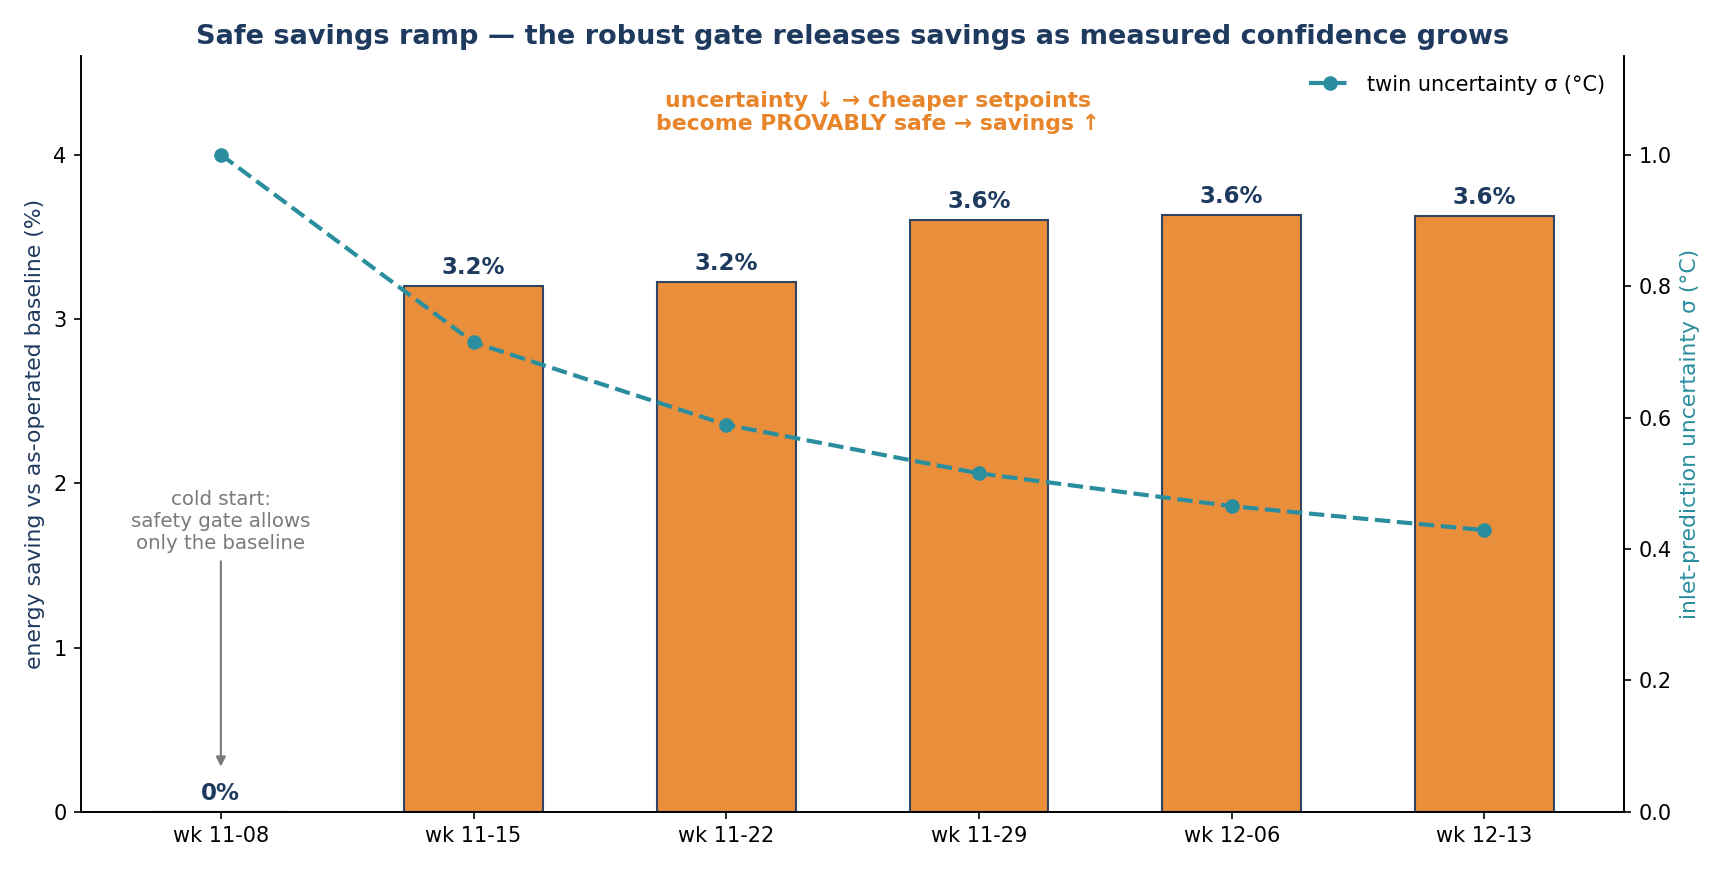
\includegraphics[width=\linewidth]{figB_savings.png}
  \caption{Safe savings ramp. Bars: per-week energy saving versus the as-operated baseline
  (\(0\rightarrow3.6\%\)). Line: the twin's inlet-prediction uncertainty \(\sigma\), falling
  from the \(1.0\,\degC\) prior toward its measured value as weeks accumulate. The robust
  gate releases savings only as the proven-safe margin grows.}
  \label{fig:savings}
\end{figure}

\paragraph{Zero violations while saving (Fig.~\ref{fig:saferecord}).} Across all six
deployed weeks there were \emph{no} inlet violations. The realized peak inlet rose toward
the cap as savings grew --- from \(23.37\,\degC\) to \(25.60\,\degC\) --- but never reached it,
leaving a worst-case margin of \(0.40\,\degC\). This is the intended behaviour: the gate
spends thermal margin only when calibrated confidence justifies it.

\begin{figure}[t]
  \centering
  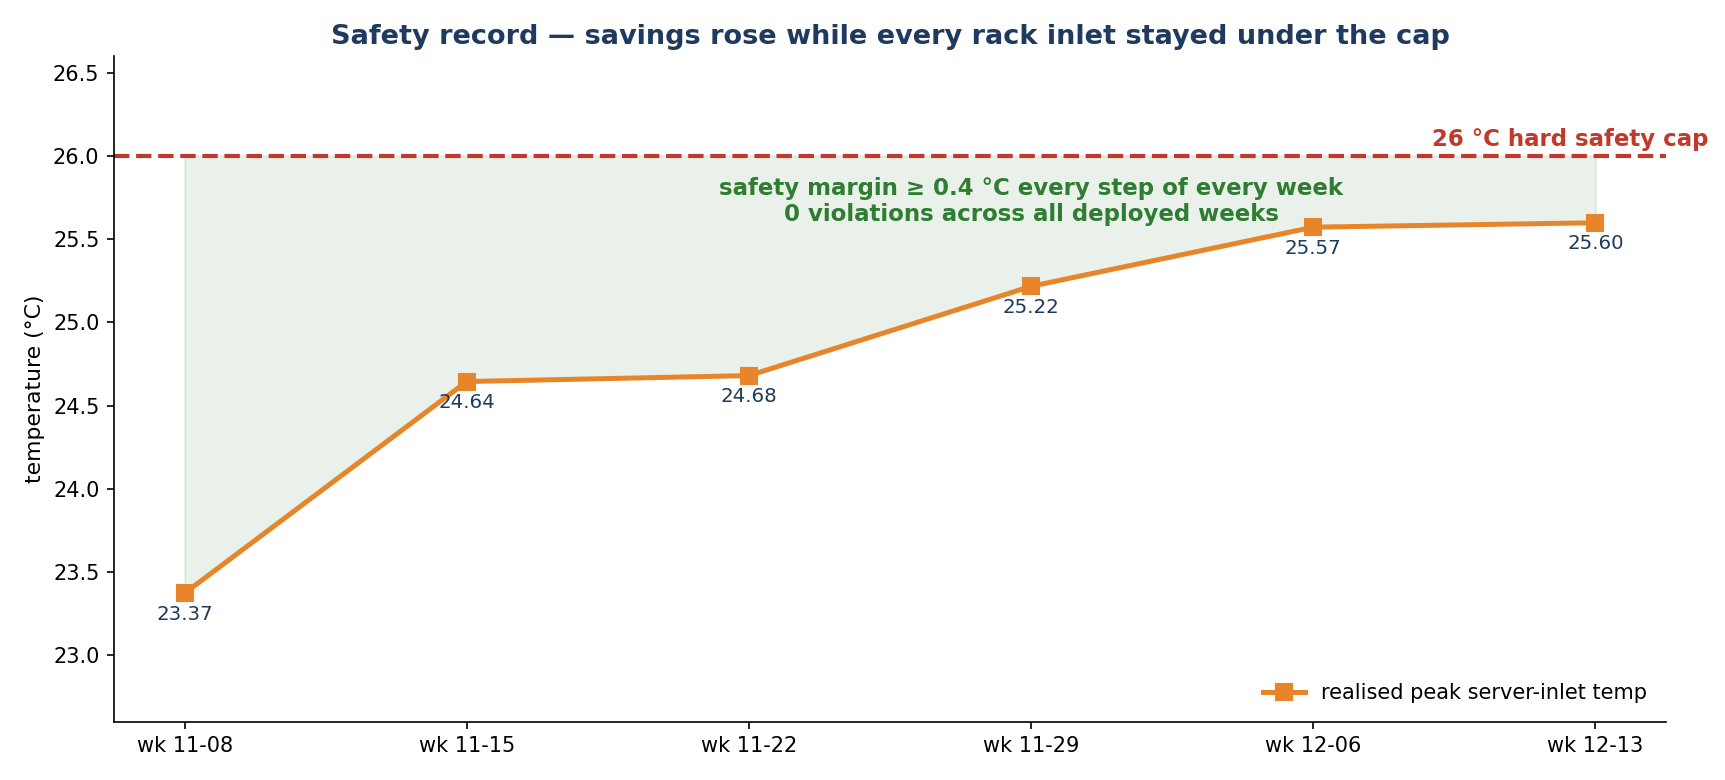
\includegraphics[width=0.92\linewidth]{figC_safety.png}
  \caption{Safety record. Realized peak server inlet per week, rising toward --- but never
  past --- the \(26\,\degC\) hard cap as savings grow; the shaded band is the realized safety
  margin. Worst realized inlet \(25.60\,\degC\); zero violations across all deployed weeks.}
  \label{fig:saferecord}
\end{figure}

\paragraph{Calibration state.} After seven paired weeks the live calibration state was a
weekly-energy bias of \(\approx515\,\mathrm{kWh}\) (\(\approx0.2\%\) of weekly energy), an
inlet bias of \(0.18\,\degC\), a fading-floor inlet \(\sigma\) of \(0.14\,\degC\), and a
posterior ensemble width \(\sigpost\) of \(0.36\,\degC\) --- the quantities that, through
Eqs.~\eqref{eq:margin} and \eqref{eq:halfwidth}, govern how aggressively the next plan may
approach the cap. The whole framework is exercised by an automated test suite (422 backend
and 104 front-end tests, plus nine Docker-gated EnergyPlus integration tests), all passing.

% =====================================================================
\section{Discussion and Limitations}
\label{sec:discussion}

The results above are deliberately reported as \emph{measured} rather than promised, and the
same honesty applies to what is \emph{not} yet field-proven. The single most important
qualifier is that the system runs in \textbf{shadow mode}: an approved plan is expanded to
the exact 45 per-actuator commands a field adapter would write, but those commands are
\emph{recorded, not actuated}. The BACnet/Modbus field adapter is an explicit, one-class
seam, and the telemetry historian is a push endpoint awaiting a real collector
(Fig.~\ref{fig:dataflow}). Consequently the ``realized'' week is a perturbed-plant
EnergyPlus simulation standing in for the building: the learning loop is \emph{structurally}
proven end-to-end, not yet \emph{field}-proven. Three further model caveats follow from
this. The recirculation correction of Eq.~\eqref{eq:recirccorr} is a provable no-op until
calibrated against real rack-inlet sensors, so the inlet margin may be optimistic for halls
with imperfect containment. The historical-analog weather \(\sigma\) of
Eq.~\eqref{eq:weatherstats} understates true synoptic extremes; the \(+1\sigma\) hot
scenario only partially compensates. And because the IT load is nearly flat in this hall,
the week-to-week story is dominated by weather, so absolute setpoints should be read as
directional until recirculation is field-calibrated.

We also deliberately scoped out humidity as a controlled variable (it is monitored and
penalized, but no dehumidification actuator is modeled), intra-week automatic re-planning
(the cadence is weekly; urgent cases are handled by cancel-and-re-plan with the live alerts
as a safety net), and end-to-end browser tests in continuous integration. None of these
changes the framework; each is additive.

The path to a field pilot is correspondingly concrete and ``config-shaped'': point a real
collector at the telemetry endpoint, implement the BACnet adapter behind the existing seam,
run in recommend-only mode for four to eight weeks comparing predictions to real
measurements, calibrate recirculation from the first real rack-inlet data, and only then
enable actuation hall-by-hall. The robustness machinery is designed to improve automatically
as real weeks accumulate: \(\sigpost\) tightens, the recalibrator re-centers the ensemble on
the believed plant, and the objective can be switched from kWh to dollars or
\(\mathrm{CO_2}\) simply by supplying the site's tariff or grid-carbon profile to
Eq.~\eqref{eq:cost}.

% =====================================================================
\section{Conclusion}
\label{sec:conclusion}

We presented a digital-twin dual-loop control framework for data-center cooling that keeps a
first-principles EnergyPlus model in the loop as the oracle on both the planning and the
deployment side, and that treats the server-inlet temperature cap as a hard constraint
defended by three independent safety nets. The inner loop searches three global setpoints
broadcast to 45 actuators, scoring each candidate by a full-week physics simulation; the
outer loop pre-validates, deploys (in shadow), measures, and learns per-KPI bias and two
uncertainties --- a fading-floor \(\sigma\) that backs the search margin and an
empirical-Bayes posterior that sizes a CVaR-based robust ensemble --- while a slower physics
recalibration corrects the plant parameters themselves. Over six consecutive deployed weeks
the twin's weekly-energy prediction error fell from \(1.33\%\) to \(0.10\%\), savings ramped
from \(0\%\) to \(3.6\%\) released strictly by earned confidence, and there were zero safety
violations (worst inlet \(25.60\,\degC\)). The remaining work to reach a live building is a
field collector and a single adapter class behind seams that already exist --- the rest of the
loop is implemented, tested, and measured today.

% =====================================================================
\section*{Reproducibility}
The framework is implemented in Python (planner and FastAPI backend) and TypeScript/React
(front end), with EnergyPlus~9.5 executed in Docker and coupled through BCVTB. Plans,
calibration state, and run artifacts are schema-versioned JSON; the per-week numbers in
Table~\ref{tab:weeks} and Figs.~\ref{fig:accuracy}--\ref{fig:saferecord} are produced
directly from the live run database and calibration history. Development followed a
test-first discipline (tests are never weakened to pass), and an automated driver reproduces
the build, smoke test, screenshot, and plan-execution steps.

% =====================================================================
\begin{thebibliography}{99}
\setlength{\itemsep}{1pt}

\bibitem{barroso} L.~A. Barroso, U.~H\"olzle, and P.~Ranganathan,
\emph{The Datacenter as a Computer: Designing Warehouse-Scale Machines}, 3rd ed.
Morgan \& Claypool, 2018.

\bibitem{greengrid} The Green Grid, ``PUE: A comprehensive examination of the metric,''
White Paper~\#49, 2012.

\bibitem{patterson} M.~K. Patterson, ``The effect of data center temperature on energy
efficiency,'' in \emph{Proc. 11th IEEE Intersociety Conf. on Thermal and Thermomechanical
Phenomena in Electronic Systems (ITherm)}, 2008, pp.~1167--1174.

\bibitem{ashrae} ASHRAE Technical Committee 9.9, \emph{Thermal Guidelines for Data
Processing Environments}, 4th ed. Atlanta, GA: ASHRAE, 2015.

\bibitem{glaessgen} E.~Glaessgen and D.~Stargel, ``The digital twin paradigm for future
NASA and U.S. Air Force vehicles,'' in \emph{53rd AIAA/ASME/ASCE/AHS/ASC Structures,
Structural Dynamics and Materials Conf.}, AIAA 2012-1818, 2012.

\bibitem{energyplus} D.~B. Crawley \emph{et al.}, ``EnergyPlus: creating a new-generation
building energy simulation program,'' \emph{Energy and Buildings}, vol.~33, no.~4,
pp.~319--331, 2001.

\bibitem{eplusref} U.S. Department of Energy, \emph{EnergyPlus Engineering Reference,
Version 9.5}. National Renewable Energy Laboratory, 2021.

\bibitem{bcvtb} M.~Wetter, ``Co-simulation of building energy and control systems with the
Building Controls Virtual Test Bed,'' \emph{Journal of Building Performance Simulation},
vol.~4, no.~3, pp.~185--203, 2011.

\bibitem{gao} J.~Gao, ``Machine learning applications for data center optimization,''
Google White Paper, 2014.

\bibitem{lazic} N.~Lazic \emph{et al.}, ``Data center cooling using model-predictive
control,'' in \emph{Advances in Neural Information Processing Systems (NeurIPS)}, 2018,
pp.~3814--3823.

\bibitem{moriyama} T.~Moriyama \emph{et al.}, ``Reinforcement learning testbed for
power-consumption optimization,'' in \emph{Methods and Applications for Modeling and
Simulation of Complex Systems (AsiaSim)}, 2018; arXiv:1808.10427.

\bibitem{rockafellar} R.~T. Rockafellar and S.~Uryasev, ``Optimization of conditional
value-at-risk,'' \emph{Journal of Risk}, vol.~2, no.~3, pp.~21--41, 2000.

\bibitem{casella} G.~Casella, ``An introduction to empirical Bayes data analysis,''
\emph{The American Statistician}, vol.~39, no.~2, pp.~83--87, 1985.

\bibitem{sharma} R.~K. Sharma, C.~E. Bash, and C.~D. Patel, ``Dimensionless parameters for
evaluation of thermal design and performance of large-scale data centers,'' in
\emph{8th AIAA/ASME Joint Thermophysics and Heat Transfer Conf.}, AIAA 2002-3091, 2002.

\end{thebibliography}

% =====================================================================
\appendix
\section{Notation and Constants}
\label{app:notation}

\begin{table}[H]
\centering
\caption{Key symbols, constants, and their values as used in the implementation.}
\label{tab:constants}
\small
\begin{tabular}{l l l}
\toprule
Symbol / quantity & Meaning & Value / range \\
\midrule
\(\Tcap\) & hard inlet-temperature cap & \(26.0\,\degC\) \\
SAT & CRAH supply-air temperature & \(20\)--\(26\,\degC\) \\
flow & CRAH supply airflow (per ACU) & \(4.8\)--\(13.8\,\mathrm{kg/s}\) \\
CHWST & chilled-water supply temperature & \(13\)--\(19\,\degC\) \\
\(\Delta t\) & control timestep & \(0.25\,\mathrm{h}\) (4/h) \\
\(T_{\mathrm{soft}}\) & inlet soft-penalty threshold & \(25.0\,\degC\) \\
\(\lambda_T,\lambda_{\mathrm{rh}},\lambda_z\) & objective penalty weights & \(1.0,\,0.2,\,0.1\) \\
\(\mathrm{RH}_{\min},\mathrm{RH}_{\max}\) & RH band & \(30\%,\,60\%\) \\
\(T^{\star}_{\mathrm{zone}}\pm b_{\mathrm{zone}}\) & zone-temperature band & \(32\pm1\,\degC\) \\
\(g,\,B,\,L\) & beam-search grid / width / levels & \(5,\,5,\,3\) \\
\(\epsilon\) & early-stop tolerance & \(10^{-3}\) \\
\(k_\sigma\) & search-margin multiplier & \(1.0\) \\
\(\alpha\) & CVaR confidence level & \(0.8\) \\
\(s_{\mathrm{base}},s_{\min}\) & ensemble half-width / floor & \(0.10,\,0.02\) \\
\(\sigma_{\mathrm{prior}}\) (inlet) & inlet uncertainty prior & \(1.0\,\degC\) \\
\(\phi\) clip & fan-efficiency correction bound & \([0.85,1.15]\) \\
\(R_{\max},\,k_r\) & recirculation cap / shortfall gain & \(0.5,\,0.5\) \\
oracle watchdog & per-candidate timeout & \(300\,\mathrm{s}\) \\
\bottomrule
\end{tabular}
\end{table}

\end{document}
